\documentclass[11pt,fleqn]{article}
\usepackage[cm]{fullpage}
%%AVC PACKAGES
\usepackage{avcgreek}
\usepackage{avcfonts}
\usepackage{avcmath}
\usepackage[numberby=section]{avcthm} % 
\usepackage{qcmacros}
\usepackage{goldstone}
%%MACROS FOR THIS DOCUMENT
\numberwithin{equation}{section}
\usepackage{titlesec}
\titleformat{\section}{\Large\bfseries\mathversion{bold}}{\thesection.}{5pt}{}
% remove header from TOC
\makeatletter
\renewcommand\tableofcontents{%
  \@starttoc{toc}%
}
\makeatother

%%%DOCUMENT%%%
\begin{document}

\title{Algebraic and Diagrammatic Methods in Electronic Structure Theory}
\author{Andreas~V.~Copan}
\date{}

\maketitle
\tableofcontents

%%TENSORS
\section{Tensors}\label{sec-tensors}

\begin{dfn}\label{covariance-contravariance-invariance}
\thmtitle{Covariance, contravariance, invariance}
Let \f be an arbitrary linear function of a vector space $V$ and consider a change of basis $\{e_1,\cd,e_n\}\rightarrow\{\tl{e}_1,\cd,\tl{e}_n\}$ defined by $\tl{e}_j = \sum_ie_i\,[\bo{T}]_{ij}$ where $\bo{T}$ is an invertible matrix.
If \f obeys the same transformation law as the basis elements, it is a \textit{covariant} quantity.
If it obeys the opposite transformation law, it is a \textit{contravariant} quatntity.
\begin{align}
&&
  \f(\tl{e}_j)=\sum_i\f(e_i)\,[\bo{T}]_{ij}
\sp\text{\textit{(covariant)}}
&&
  \f(\tl{e}_i)=\sum_j[\bo{T}^{-1}]_{ij}\,\f(e_j)
\sp\text{\textit{(contravariant)}}
\end{align}
\textit{Covariant} quantities are typically denoted with subscript indices, $\f_i=\f(e_i)$, whereas \textit{contravariant} quantities are denoted with superscript indices, $\f^i=\f(e_i)$.
Abstract quantities such as vectors and operators are called \textit{invariant}, since they do not depend on the choice of basis.
\end{dfn}

\begin{ex}\label{vector-coordinates-are-contravariant}
\thmtitle{Vector coordinates are contravariant}
Let $\{v_i\}$ be the coordinates of a vector $v$ in the basis $\{e_i\}$, and let $\{\tl{v}_j\}$ be its coordinates in $\{\tl{e}_j=\sum_ie_i\,[\bo{T}]_{ij}\}$.
Then the invariance of $v$ implies that the coordinates are contravariant:
\begin{align*}
  \sum_ie_iv_i=v=\sum_j\tl{e}_j\tl{v}_j
=
  \sum_ie_i\sum_j[\bo{T}]_{ij}\tl{v}_j
\implies
  v_i
=
  \sum_j[\bo{T}]_{ij}\tl{v}_j
\implies
  \tl{v}_j
=
  \sum_i[\bo{T}^{-1}]_{ji}v_i
\end{align*}
Therefore, vector coordinates should be written with superscript indices $v_i\mapsto v^i$.
\end{ex}

\begin{dfn}
\thmtitle{Linear functional}
A \textit{linear functional} $f:V\rightarrow\mb{C}$ is a scalar-valued function on $V$ that satisfies $f(v+w)=f(v)+f(w)$ and $f(cv)=cf(v)$ for all $c\in\mb{C}$ and all $v,w\in V$.
The \textit{null functional} is given by $f_0(v)=0\ \forall v\in V$.
\end{dfn}

\begin{dfn}
\thmtitle{Dual space $V^*$}
The \textit{dual space} of $V$, denoted $V^*$, is the space of linear functionals on $V$, which itself forms a vector space with respect to vector addition $(f+g)\in V^*$ and scalar multiplication $(cf)\in V^*$ defined by
\begin{align}
&&
  (f+g)(v)
\equiv
  f(v) + g(v)
&&
  (cf)(v)
\equiv
  cf(v)
\end{align}
for all $f,g\in V^*$, $v\in V$, and $c\in\mb{C}$.
Its dimension is $\dim V^*=\dim V$, which follows from \Cref{canonical-dual-basis}.
\end{dfn}

\begin{prop}\label{canonical-dual-basis}
\thmtitle{The canonical dual basis}
\thmstatement{If $\{e_1,\cd,e_n\}$ is a basis for $V$ then $\{e^1,\cd,e^n\}\subset V^*$, defined by $e^i(e_j)=\d^i_j$, is a basis for $V^*$.
This ``canonical dual basis'' transforms contravariantly relative to $\{e_1,\cd,e_n\}$. }
\thmproof{
  First, note that $e^j(v)=e^j(\sum_ie_iv^i)=\sum_ie^j(e_i)v^i=v^j$ for any $v\in V$.
  Therefore, $f(v)=f(\sum_ie_iv^i)=\sum_if(e_i)v^i=\sum_if(e_i)e^i(v)$ holds for all $f\in V^*$ and all $v\in V$, which implies that $f=\sum_if(e_i)e^i$.
  This shows that $\spn\{e^1,\cd,e^n\}=V^*$.
  Second, assume there exist $c_j\in\mb{C}$ such that $\sum_jc_je^j=f_0$, where $f_0$ is the null functional.
  Then $0=f_0(e_i)=\sum_jc_je^j(e_i)=c_i$ and all of the coefficients must be zero, showing that $\{e^1,\cd,e^n\}$ is linearly independent.
  Since both sets have $n$ elements, $\dim V=\dim V^*$.
  Since $v^j=e^j(v)$, the dual basis is contravariant.
}
\end{prop}

\begin{rmk}
If $\ip{\cdot|\cdot}$ is an inner product on $V$ and $\bo{S}$ is the matrix of overlaps, $\ip{e_i|e_j}=[\bo{S}]_{ij}$, then the canonical dual basis is given by $e^i(\cdot)=\sum_j[\bo{S}^{-1}]_{ij}\,\ip{e_j|\cdot}$, which simplifies to $e^i(\cdot)=\ip{e_i|\cdot}$ when $\{e_1,\cd,e_n\}$ is orthonormal.
\end{rmk}

\begin{dfn}
\thmtitle{Linear operator}
A \textit{linear operator} $\op{T}:V\rightarrow V$ is a vector-valued function on $V$ that satisfies $\op{T}(v+w)=\op{T}v + \op{T}w$ and $\op{T}(cv)=c\op{T}v$.
The \textit{identity operator} is given by $\op{1}v=v$ and the \textit{null operator} is given by $\op{0}v=v$.
\end{dfn}

\begin{prop}\label{resolution-of-the-identity}
\thmtitle{Resolution of the identity}
\thmstatement{Given a basis $\{e_i\}$, the identity operator can be expressed as $\op{1}=\sum_ie_ie^i$.}
\thmproof{
  $\op{1}(v)=v=\sum_ie_iv^i=\sum_ie_ie^i(v)$ holds for all $v\in V$ (see \Cref{canonical-dual-basis}), so $\op{1}=\sum_ie_ie^i$.
}
\end{prop}

\begin{rmk}
Using \Cref{resolution-of-the-identity}, we can identify the matrix of a linear operator, $\op{T}e_j=\sum_ie_i\,[\bo{T}]_{ij}$, with $[\bo{T}]_{ij}=e^i(\op{T}e_j)$.
Therefore, the row index of $\bo{T}$ should be written as a superscript index, $[\bo{T}]_{ij}\mapsto[\bo{T}]^i_j$.
Using two resolutions of the identity, $\op{T}$ can be expressed as $\op{T}=\sum_{ij}[\bo{T}]_j^ie_ie^j$, which identifies $\bo{T}$ as its coordinates in $V\times V^*=\spn\{e_ie^j\}$.
\end{rmk}

\begin{rmk}
The formula for matrix multiplication also follows from \Cref{resolution-of-the-identity}:
the matrix of $\op{T}\op{T}'$ is $e^i(\op{T}\op{T}'e_j)=\sum_ke^i(\op{T}e_k)e^k(\op{T}'e_j)=\sum_k[\bo{T}]^i_k[\bo{T}']^k_j$.
\end{rmk}

\begin{dfn}\label{direct-sum-v-oplus-v'}
\thmtitle{Direct sum $V\oplus V'$}
A \textit{direct sum} of vector spaces $V$ and $V'$ is $V\oplus V'\equiv\{v\oplus v'\,|\,v\in V,\,v'\in V'\}$, a new vector space with vector addition and scalar multiplication defined by
\begin{align}
&&
  v_1\oplus v_1'
+
  v_2\oplus v_2'
=
  (v_1 + v_2)
\oplus
  (v_1' + v_2')
&&
  c(v\oplus v')
=
  cv\oplus cv'\,.
\end{align}
If $\{e_i\}$ and $\{e_{i'}'\}$ are bases for $V$ and $V'$ then $\{e_i\oplus0'\}\cup\{0\oplus e_{i'}'\}$ is a basis for $V\oplus V'$, which has dimension $\dim V+\dim V'$.
\end{dfn}

\begin{dfn}\label{tensor-product-v-otimes-v'}
\thmtitle{Tensor product $V\otimes V'$}
A \textit{tensor product} of vector spaces $V$ and $V'$ is $V\otimes V'\equiv\{\sum v\otimes v'\,|\,v\in V,\,v'\in V'\}$, a new vector space with vector addition and scalar multiplication defined by
\begin{align}
&&
  v_1\otimes v'
+
  v_2\otimes v'
=
  (v_1 + v_2)\otimes v'
&&
  v\otimes v_1'
+
  v\otimes v_2'
=
  v\otimes(v_1' + v_2')
&&
  c(v\otimes v')
=
  (cv)\otimes v'
=
  v\otimes(cv')
\end{align}
If $\{e_i\}$ and $\{e_{i'}'\}$ are bases for $V$ and $V'$ then $\{e_i\otimes e_{i'}'\}$ is a basis for $V\otimes V'$, which has dimension $\dim V\cdot\,\dim V'$.
\end{dfn}

\begin{rmk}
Since the sum $S+S'$ of two mutually orthogonal subspaces $S, S\subseteq V$ is isomorphic to their direct sum, $S\oplus S'$ and $S+S'$ are used interchangeably in this context.
The reverse is also true.
The direct sum of two distinct vector spaces $V\oplus V'$ contains copies of $V$ and $V'$ as mutually orthogonal subspaces, namely $V\simeq V\oplus0'$ and $V'\simeq 0\oplus V'$.
\end{rmk}

\begin{dfn}
\thmtitle{Direct sums and tensor products of inner product spaces}
If $V$ and $V'$ are inner product spaces, then $V\oplus V'$ and $V\otimes V'$ are also inner product spaces with respect to the following inner products.
\begin{align}
&&
  \ip{v\oplus v'|w\oplus w'}_{V\oplus V'}
\equiv
  \ip{v|w}_V
+
  \ip{v'|w'}_{V'}
&&
  \ip{v\otimes v'|w\otimes w'}_{V\otimes V'}
\equiv
  \ip{v|w}_V
\cdot
  \ip{v'|w'}_{V'}
\end{align}
\end{dfn}

\begin{dfn}\label{tensor}
\thmtitle{Tensor}
A \textit{tensor} is a vector in a tensor product space.
An \textit{n\eth order tensor} lives in a product of $n$ vector spaces, $V_1\otimes\cdots\otimes V_n$.
A \textit{type-(m,n) tensor on $V$} lives in $\underset{\text{$m$ times}}{V\otimes\cdots\otimes V}\otimes \underset{\text{$n$ times}}{V^*\otimes\cdots \otimes V^*}$, denoted $T_n^m(V)$.
\end{dfn}

\begin{ex}
$T_0^0(V)$ is the scalar field \mb{C},
$T_0^1(V)$ is the vector space itself, $T_1^0(V)$ is the dual space $V^*$, and $T_1^1(V)$ is (up to isomorphism) the space of linear operators $V\otimes V^*\simeq V\times V^*$.
\end{ex}

\begin{rmk}
A member $t$ of $T_n^m(V)$ can be expanded in the basis $\{e_1,\cd,e_n\}$ as follows.
\begin{align}
&&
  t
=
  \sum_{\substack{i_1\cdots i_m\\j_1\cdots j_n}}
  t_{j_1\cdots j_n}^{i_1\cdots i_m}
  e_{i_1}\otimes\cdots\otimes e_{i_m}\otimes e^{j_1}\otimes\cdots\otimes e^{j_n}
\end{align}
Its coordinate array $\bo{t}=[t^{i_1\cdots i_m}_{j_1\cdots j_n}]$ is indexed by $m$ contravariant indices and $n$ covariant indices.
\end{rmk}

\begin{rmk}
Just as people often use the term ``vector'' to refer to the basis-dependent coordinate array $v^i$ rather than $v$ itself, more often than not the word ``tensor'' refers to the coordinate array $t^{i_1\cdots i_m}_{j_1\cdots j_n}$ rather than the abstract quantity $t$.
\end{rmk}

\begin{dfn}
\thmtitle{Tensor product $t\otimes t'$}
The \textit{tensor product} of $t\in T_n^m(V)$ and $t'\in T_{n'}^{m'}(V)$ is $t\otimes t'\in T_{n+n'}^{m+m'}(V)$ with coordinate array $[\bo{t}\otimes \bo{t}']_{j_1\cd j_{n+n'}}^{i_1\cd i_{m+m'}} = t_{j_1\cd j_n}^{i_1\cd i_m}t_{j_{n+1}\cd j_{n+n'}}^{i_{m+1}\cd i_{m+m'}}$.
This generalizes the \textit{matrix Kronecker product}.
\end{dfn}

\begin{dfn}
\thmtitle{Tensor contraction}
A \textit{(p,q) tensor contraction} is a map $\tr_{p,q}:T_n^m(V)\rightarrow T_{n-1}^{m-1}(V)$ given by tracing the $p\eth$ element in $V$ with the $q\eth$ element in $V^*$:
\begin{align}
&&
  \tr_{p,q}\pr{
    e_{i_1}\otimes\cd\otimes e_{i_p}\otimes\cd\otimes e^{j_q}\otimes\cd\otimes e^{j_n}
  }
=
  \d_{i_p}^{j_q}\,
  e_{i_1}\otimes\cd\otimes \cancel{e_{i_p}}\otimes\cd\otimes 
  \cancel{e^{j_q}}\otimes\cd\otimes e^{j_n}
\end{align}
The coordinate array of $\tr_{p,q}(t)$ is $[\tr_{p,q}(\bo{t})]^{i_1\cd \cancel{i_p}\cd i_m}_{j_1\cd \cancel{j_q}\cd j_m}=\sum_{i_p,j_q}\d_{i_p}^{j_q}\,t^{i_1\cd i_m}_{j_1\cd j_m}$, generalizing the \textit{matrix trace}, $\tr(M)=\sum_i M_i^i$.
\end{dfn}

\begin{dfn}
\thmtitle{Cross-contraction}
A \textit{cross-contraction} traces a lower index on one tensor with an upper index on another, $\tr_{p,q'}:T_n^m(V)\otimes T_{n'}^{m'}(V)\rightarrow T^{m}_{n-1}(V)\otimes T^{m'-1}_{n'}$, generalizing the \textit{matrix product} $\tr_{1,1'}(M\otimes M')=\sum_k M^i_kM^k_j$.
\end{dfn}

\begin{ntt}\label{einstein-summation}
\thmtitle{Einstein summation convention}
In the \textit{Einstein summation convention} any index which appears twice in a product, once as a covariant index and once as a contravariant one, is implicitly summed over: $\sum_i a_i b^i\mapsto a_ib^i$.
For most purposes, this rule suffices to dispense with summation symbols altogether.
The basis expansion of a vector now takes the form $v=e_iv^i$, that of a tensor takes the form $t = t_{j_1\cd j_n}^{i_1\cd i_m}e_{i_1}\otimes\cd\otimes e_{i_m}\otimes e^{j_1}\otimes\cd\otimes e^{j_n}$, and resolution of the identity can be written as $\op{1}=e_ie^i$.
The choice of symbol for a \textit{contracted index} is is arbitrary, wherease each \textit{free \emph{(uncontracted)} index} symbol must appear once in every term on the right- and left-hand sides of an equation, always with the same co- or contra-variance.
\end{ntt}

\begin{ex}
In Einstein notation, the matrix expression $\bo{C}=\bo{A}\bo{B}$ is written as $C^i_j=A^i_kB^k_j$.
\end{ex}

\begin{ex}
The expression
$a_{ij}^{kl}=\tfr{1}{2}b_{ij}^{vx}c_{vx}^{kl}+\tfr{1}{6}d_{ijv}^{xyz}e_{xyz}^{klv}$ is a balanced equation with free indices $\substack{kl\\ij}$.
Each term is an element of $T_2^2(V)$, so the addition $(+)$ and assignment $(=)$ operations are well-defined.
\end{ex}



\newpage
\section{Fock space}

\subsection{Position-space representation}

\begin{dfn}
\thmtitle{$n$-electron Hilbert space}
If $\mc{H}$ is a complete one-electron Hilbert space and $\{\y_p\}$ is its spin-orbital basis, then $\mc{H}^{\otimes n}=\underset{\text{$n$ times}}{\mc{H}\otimes\cd\otimes\mc{H}}=\spn\{\y_{p_1}\otimes\cd\otimes\y_{p_n}\}$ is an \textit{$n$-electron Hilbert space}.
The inner product on $\mc{H}^{\otimes n}$ is
\begin{align}
&&
  \ip{\y_{p_1}\otimes\cd\otimes\y_{p_n}|\y_{q_1}\otimes\cd\otimes\y_{q_n}}
=
  \ip{\y_{p_1}|\y_{q_1}}\cd\ip{\y_{p_n}|\y_{q_n}}\,.
\end{align}
Projection onto $\br{1\otimes\cd\otimes n}$, where $\kt{i}=\kt{\bo{r}_i,s_i}$ is a space-spin electronic state, reveals that the basis states $\y_{p_1}\otimes\cd\otimes\y_{p_n}$ are abstact representations of ordinary product states, $\ip{1\otimes\cd\otimes n|\y_{p_1}\otimes\cd\otimes\y_{p_n}}=\y_{p_1}(1)\cd\y_{p_n}(n)$.
\end{dfn}

\begin{dfn}\label{slater-determinant}
\thmtitle{$n$-electron Slater determinant}
An \textit{$n$-electron Slater determinant} $\F_{(p_1\cd p_n)}$ is a normalized antisymmetric product of $n$ one-electron states $\y_{p_1},\cd,\y_{p_n}$
\begin{align}
&&
  \F_{(p_1\cd p_n)}
=
  \tfr{1}{\sqrt{n!}}
  \sum_{\pi\in\mr{S}_n}
  \e_{\pi}
  \y_{p_{\pi(1)}}\otimes\cd\otimes\y_{p_{\pi(n)}}
\end{align}
where $\pi\in\mr{S}_n$ is a permutation of $1\cd n$ and $\e_{\pi}$ is $(-)^{\text{\# transpositions}}$.
Projecting into position space yields its familiar form.
\begin{align*}
&&
  \ip{1\otimes\cd\otimes n|\F_{(p_1\cd p_n)}}
=
  \F_{(p_1\cd p_n)}(1,\cd,n)
=
  \tfr{1}{\sqrt{n!}}
  \det|\y_{p_{\pi(1)}}(1)\cd\y_{p_{\pi(n)}}(n)|
\end{align*}
\end{dfn}

\begin{rmk}\label{direct-derivation-of-second-quantization}
\thmtitle{A direct derivation of second quantization in position-space representation}
Let $F_n$ be the space of $n$-electron Slater determinants, $\F_{(p_1\cdots p_n)}$, a subspace of $\mc{H}^{\otimes n}$.
Consider the integral operator $\op{a}_p:F_n\rightarrow F_{n-1}$ given by
\begin{align}
&&
  \Y(1,\cd,n)
\mapsto
  (\op{a}_p\Y)(2,\cd,n)
\equiv
  \sqrt{n}\int d(1) \y_p^*(1)\Y(1,2,\cd,n)\,.
\end{align}
This operator acts on Slater determinants as
\begin{align*}
  (\op{a}_p\F_{(p_1\cd p_n)})(2,\cd,n)
=
  \tfr{1}{\sqrt{(n-1)!}}
  \sum_{\pi\in\mr{S}_n}
  \ip{\y_p|\y_{p_{\pi(1)}}}
  \y_{p_{\pi(2)}}(2)\cd\y_{p_{\pi(n)}}(n)
=
\left\{
\ar{
  (-)^{k-1}\F_{(p_1\cd \cancel{p_k}\cd p_n)} & p=p_k\in(p_1\cd p_n)\\[5pt]
  0 & \text{otherwise}
}
\right.
\end{align*}
i.e. it deletes the orbital $\y_p$ from $\F_{(p_1\cd p_n)}$ if exists and otherwise kills the determinant.
The restriction of $\op{a}_p$ to the space of antisymmetric functions implies that these operators anticommute, $\op{a}_p\op{a}_q=-\op{a}_q\op{a}_p$, since
\begin{align*}
  \int d(1)d(2)\y_p^*(1)\y_q^*(2)\Y(1,2,\cd,n)
=
  \int d(1)d(2)\y_q^*(1)\y_p^*(2)\Y(2,1,\cd,n)
=
-
  \int d(1)d(2)\y_q^*(1)\y_p^*(2)\Y(1,2,\cd,n)
\end{align*}
by changing dummy variables of integration and plugging in $\Y(2,1,\cd,n)=-\Y(1,2,\cd,n)$.
These deletion operators provide the following decomposition of functions in $F_n$.
\begin{align}
&&
  \Y(1,\cd,n)
=
  \tfr{1}{\sqrt{n}}
  \sum_p^\infty\y_p(1)\pr{\op{a}_p\Y}(2,\cd,n)
=
  \tfr{1}{\sqrt{n(n-1)}}
  \sum_{pq}^\infty
  \y_p(1)\y_q(2)(\op{a}_q\op{a}_p\Y)(3,\cd,n)
\end{align}
Therefore, general matrix elements of the electronic Hamiltonian with respect to $\Y,\Y'\in F_n$ can be expressed as
\begin{align*}
  \ip{\Y|\op{H}_e\Y'}
=
  \sum_{i=1}^n\ip{\Y|\op{h}(i)\Y'}
+
  \sum_{i<j}^n\ip{\Y|\op{g}(i,j)\Y'}
=&\
  n\ip{\Y|\op{h}(1)\Y'}
+
  \tfr{n(n-1)}{2}
  \ip{\Y|\op{g}(1,2)\Y'}
\\=&\
  \sum_{pq}^\infty
  h_{pq}\ip{\op{a}_p\Y|\op{a}_q\Y'}
+
  \tfr{1}{2}
  \sum_{pqrs}^\infty
  \ip{pq|rs}\ip{\op{a}_q\op{a}_p\Y|\op{a}_s\op{a}_r\Y'}
\end{align*}
where $\op{h}(i)\equiv-\tfr{1}{2}\nabla_i^2+\sum_A\tfr{Z_A}{|\bo{r}_i-\bo{R}_A|}$, $\op{g}(i,j)\equiv\tfr{1}{|\bo{r}_i-\bo{r}_j|}$, $h_{pq}\equiv\ip{\y_p(1)|\op{h}(1)\y_q(1)}$, and $\ip{pq|rs}\equiv\ip{\y_p(1)\y_q(2)|\op{g}(1,2)\y_r(1)\y_s(2)}$.
Therefore, restricting $\op{H}_e$ to the space of physically realistic (i.e.~antisymmetric) functions, we get the following identity
\begin{align}\label{second-quantized-hamiltonian}
&&
  \op{H}_e
=
  \sum_{pq}^\infty
  h_{pq}
  \op{a}_p\dg \op{a}_q
+
  \tfr{1}{2}
  \sum_{pqrs}^\infty
  \ip{pq|rs}
  \op{a}_p\dg\op{a}_q\dg\op{a}_s\op{a}_r
\end{align}
which is the \textit{second quantized} form of the Hamiltonian, as opposed to the \textit{first quantized} form which is not restricted to antisymmetric functions.
A defining feature of the second quantization formalism is that $\op{H}_e$ is independent of the number of electrons.
\end{rmk}


\subsection{Abstract representation}

\begin{dfn}\label{fock-space}
\thmtitle{Fock space}
Let $F_n(\mc{H})$ denote $\spn\{\F_{(p_1\cd p_n)}\}$, the antisymmetric subspace of $\mc{H}^{\otimes n}$.
The fermionic \textit{Fock space} is the union of all of these spaces, $F(\mc{H})=F_0(\mc{H})\oplus F_1(\mc{H})\oplus F_2(\mc{H})\oplus\cd\oplus F_{\infty}(\mc{H})$, which comprises all possible electronic wavefunctions.
\end{dfn}

\begin{dfn}\label{occupation-number-representation}
\thmtitle{The occupation number representation of $F(\mc{H})$}
In the \textit{occupation number representation} of Fock space, the basis vectors are represented as lists of 1s and 0s,
$
  \kt{\bo{n}}
\equiv
  \kt{n_1,n_2,n_3,\cd,n_\infty}
$,
where $n_p=1$ when $\y_p$ is occupied and $n_p=0$ when $\y_p$ is unoccupied in the state.
One possible basis for $F(\mc{H})$ is given by distributing 1s and 0s over the occupation vector in all possible ways.
The state in which no spin-orbitals are occupied is called the \textit{vacuum state}, denoted $\kt{\vac}$, which spans $F_0(\mc{H})\simeq\mb{C}$.
\end{dfn}

\begin{dfn}\label{particle-hole-operators}
\thmtitle{Particle-hole operators}
\textit{Particle-hole operators} change the occupation numbers of one-particle states.
The \textit{annihilation operator} of $\y_p$ is a linear mapping $a_p:F_n(\mc{H})\rightarrow F_{n-1}(\mc{H})$ defined by
\begin{align}
&&\label{occ-num-annihilation-operator-action}
  a_p\kt{\cd n_p\cd}
=
  (-)^{n_1+\cd+n_{p-1}}
  \kt{\cd n_p-1\cd}
\ \ \ \text{if $n_p=1$}
&&
  a_p\kt{\cd n_p\cd}
=
  0
\ \ \ \text{if $n_p=0$}
\end{align}
and the \textit{creation operator} of $\y_p$ is a linear mapping $c_p:F_n(\mc{H})\rightarrow F_{n+1}(\mc{H})$ defined by
\begin{align}
&&\label{occ-num-creation-operator-action}
  c_p\kt{\cd n_p\cd}
=
  (-)^{n_1+\cd+n_{p-1}}
  \kt{\cd n_p+1\cd}
\ \ \ \text{if $n_p=0$\ }
&&
  c_p\kt{\cd n_p\cd}
=
  0
\ \ \ \text{if $n_p=1$.}
\end{align}
\end{dfn}

\begin{prop}
\thmtitle{$c_p=a_p\dg$}
\thmstatement{Creation and annihilation operators of the same state $\y_p$ are adjoints of each other.}
\thmproof{
  $\ip{n_1'n_2'\cd|a_p[n_1n_2\cd]}$ vanishes unless $n_p'=0$, $n_p=1$, and $n_q'=n_q\ \forall q\neq p$.
  Likewise for $\ip{c_p[n_1'n_2'\cd]|n_1n_2\cd}$.
  Therefore, $\ip{\Y|a_p\Y'}=\ip{c_p\Y|\Y'}$ for all $\Y,\Y'\in F(\mc{H})$ and $c_p=a_p\dg$ by the definition of adjoint.
}
\end{prop}

\begin{prop}\label{particle-hole-operator-anticommutator}
\thmtitle{$[q,q']_+=\d_{q'q\dg}$}
\thmstatement{Particle-hole operators $q$ and $q'$ anticommute unless $q'=q\dg$, for which $[q,q\dg]_+=1$.}
\thmproof{
  Let $q$ and $q'$ be arbitrary particle-hole operators acting on $\y_p$ and $\y_{p'}$, respectively.
  First, suppose $p\neq p'$. Then
  \begin{align*}
  &
    qq'\kt{\cd n_p\cd n_{p'}\cd}
  =
    (-)^{n_p+\sum_{r=p+1}^{p'}n_r}
    \kt{\cd\ol{n_p}\cd\ol{n_{p'}}\cd}
  \,\text{, and}
  \\
  &
    q'q\kt{\cd n_p\cd n_{p'}\cd}
  =
    (-)^{\ol{n_p}+\sum_{r=p+1}^{p'}n_r}
    \kt{\cd\ol{n_p}\cd\ol{n_{p'}}\cd}
  \end{align*}
  where $\ol{n_p}$ and $\ol{n_{p'}}$ are the occupations after applying $q$ and $q'$.
  Since $n_p$ and $\ol{n_p}$ differ by one, $qq'=-q'q$.
  The second case, $p=p'$, implies $q'\in\{q,q\dg\}$.
  If $q'=q$, then $qq'=-q'q=0$.
  If $q'=q\dg$, either $n_p=1\implies(a_p\dg a_p + a_pa_p\dg)\kt{\cd n_p\cd}=(1+0)\kt{\cd n_p\cd}$ or $n_p=0\implies(a_p\dg a_p + a_pa_p\dg)\kt{\cd n_p\cd}=(0+1)\kt{\cd n_p\cd}$.
  Either way, $q'=q\dg\implies(qq' + q'q)=1$.
}
\end{prop}

\begin{rmk}
\thmtitle{Relating the determinant and occupation number representations}
When $p_1<\cd<p_n$, $\F_{(p_1\cd p_n)}$ is equivalent to the occupation vector $\kt{\bo{n}_{(p_1\cd p_n)}}$ with 1s at $p_1,\cd,p_n$.
Otherwise, this determinant is equivalent to $\e_{\pi}\kt{\bo{n}_{(p_1\cd p_n)}}$ for $\pi\in\mr{S}_n$ such that $p_{\pi(1)}<\cd<p_{\pi(n)}$.
The actions of $a_p$ and $a_p\dg$ on $\F_{(p_1\cd p_n)}$ are given by
\begin{align}
&&\label{abstract-annihilation-operator-action}
  a_p\F_{(p_1\cd p_n)}
=
  (-)^{k-1}\F_{(p_1\cd\cancel{p_k}\cd p_n)}
  \ \text{if $p=p_k\in(p_1\cd p_n)$}
&&
  a_p\F_{(p_1\cd p_n)}
=
  0
  \ \text{if $p\notin(p_1\cd p_n)$}
\\\label{abstract-creation-operator-action}
&&
  a_p\dg\F_{(p_1\cd p_n)}
=
  (-)^{k-1}\F_{(p_1\cd p_{k-1}pp_k\cd p_n)}
  \ \text{if $p\notin(p_1\cd p_n)$}
&&
  a_p\dg\F_{(p_1\cd p_n)}
=
  0
  \ \text{if $p\in(p_1\cd p_n)$}
\end{align}
which follows directly from \Cref{occ-num-annihilation-operator-action,occ-num-creation-operator-action} when $p_1<\cd<p_n$.
Other cases follow from the fact that any sign factors for permuting $(p_1\cd p_n)$ cancel on both sides of the equation, including the position of insertion or deletion, $p_k$, whose phase is tracked by $(-)^{k-1}$ on the right.
That is, both sides of the equation are antisymmetric to permutations of $(1\cd n)$.
Note that \Cref{abstract-annihilation-operator-action} was also derived in \Cref{direct-derivation-of-second-quantization} using the position-space representation of $a_p$.
One advantage of the determinant basis is that, unlike occupation vectors, determinants translate directly into strings of creations operators
\begin{align}
&&
  \kt{\F_{(p_1\cd p_n)}}
=
  a_{p_1}\dg\cd a_{p_n}\dg\kt{\vac}
\end{align}
without any phase ambiguity.
Together with the second quantized form of the electronic Hamiltonian (\Cref{second-quantized-hamiltonian}), this boils much of the grunt work of electronic structure theory down to particle-hole operator algebra.
\end{rmk}

\begin{dfn}
\thmtitle{Excitation operators and excited determinants}
Operator strings of the form $a_{p_1}\dg\cd a_{p_m}\dg a_{q_m}\cd a_{q_1}$ are called \textit{excitation operators}.
For a given reference determinant $\F$, excited determinants can be constructed as
\begin{align}
&&
  \F_{i_1\cd i_m}^{a_1\cd a_m}
=
  a_{a_1}\dg\cd a_{a_m}\dg a_{i_m}\cd a_{i_1}\F
=
  a_{a_1}\dg a_{i_1}\cd a_{a_m}\dg a_{i_m}\F
\end{align}
where $i_1,\cd,i_m$ are occupied and $a_1,\cd,a_m$ are virtual indices with respect to $\F$.
\end{dfn}


\section{\vac-normal ordering}

\begin{dfn}
\thmtitle{\vac-normal order}
A string $q_1\cd q_n$ of particle-hole operators is in \textit{\vac-normal order} when all of its creation operators sit to the left of its annihilation operators.
That is, a \vac-normal string has the form $a_{p_1}\dg\cd a_{p_m}\dg a_{r_1}\cd q_{r_{m'}}$.
This form guarantees that the vacuum expectation value of the string goes to zero, $\ip{\vac|q_1\cd q_n|\vac}=0$.
\end{dfn}

\begin{dfn}
\thmtitle{\vac-normal ordering}
The \textit{\vac-normal ordering} of a string $q_1\cd q_n$ of particle-hole operators is the mapping $q_1\cd q_n\mapsto\no{q_1\cd q_n}\equiv\e_{\pi}q_{\pi(1)}\cd q_{\pi(n)}$ where $\pi\in\mr{S}_n$ is a permutation that places the string in normal order.
\end{dfn}

\begin{dfn}\label{vac-normal-contraction}
\thmtitle{\vac-normal contraction}
A \textit{\vac-normal contraction} of two particle particle-hole operators $q_1$ and $q_2$ is defined as $\ctr{}{q}{_1}{q}q_1q_2\equiv q_1q_2 - \no{q_1q_2}$.
This associates a scalar value with every pair in $\{a_p\}\cup\{a_p\dg\}$, of which only
$\ctr{}{a}{_p}{a} a_pa_q\dg=a_pa_q\dg - \no{a_pa_q\dg}=[a_p,a_q\dg]_+=\d_{pq}$
is non-zero.
\end{dfn}

\begin{dfn}
\thmtitle{n\eth order density moments}
The \textit{$m\eth$ order density moment} of a series of particle-hole operators $q_1,\cd,q_m$ is the statistical average of their product, $\ip{\Y|q_1\cd q_m|\Y}$, with respect to a reference state $\Y\in F(\mc{H})$.
\end{dfn}

\begin{dfn}
\thmtitle{One-particle and one-hole density matrices}
For a state $\Y\in F_n(\mc{H})$ with a definite particle count, the lowest-order non-vanishing density moments are $\g_{pq}\equiv\ip{\Y|a_q\dg a_p|\Y}$ and $\h_{pq}\equiv\ip{\Y|a_pa_q\dg|\Y}$, the \textit{one-particle} and \textit{one-hole density matrices}.
\end{dfn}

\begin{rmk}
\thmtitle{\vac-normal contractions as pairwise density moments of the vacuum}
\vac-normal contractions can be identified with pairwise moments of the vacuum state via $\ctr{}{q}{_1}{q}q_1q_2=\ip{\vac|q_1q_2-\no{q_1q_2}|\vac}=\ip{\vac|q_1q_2|\vac}$, since $\ip{\vac|\no{q_1q_2}|\vac}=0$ by definition and $\ctr{}{q}{_1}{q}q_2q_2$ is a scalar quantity.
The only non-vanishing \vac-normal contractions are elements of the \vac one-hole density matrix, $\ctr{}{a}{_p}{a}a_pa_q\dg=\ip{\vac|a_pa_q\dg|\vac}=\h_{pq}$, which evaluates to $\d_{pq}$.
\end{rmk}

\begin{ntt}
\thmtitle{\vac-normal-ordered strings with contraction lines}
Let the notation $\no{q_1\cd\ctr{}{q}{_i\cd}{q}q_i\cd q_j\cd q_n}$ stand for
\begin{align}
&&
  \no{q_1\cd\ctr{}{q}{_i\cd}{q}q_i\cd q_j\cd q_n}
\equiv
  (-)^{j-i-1}\ctr{}{q}{_i}{q}q_iq_j\no{q_1\cd\cancel{q_i}\cd\cancel{q_j}\cd q_n}
\end{align}
where the phase factor corresponds to the signature of the permutation required to join $q_i$ and $q_j$.  The same rule applies for \vac-normal-ordered strings with multiple contraction lines.
\end{ntt}

\begin{prob}\label{wick-example}
Using only the anticommutator relation of \Cref{particle-hole-operator-anticommutator}, show that $a_pa_qa_s\dg a_r\dg$ can be expanded into the following linear combination of operator \vac-normal operator strings.
\begin{align*}
  a_pa_qa_s\dg a_r\dg
=&\
  a_s\dg a_r\dg a_pa_q
+
  \d_{ps} a_r\dg a_q
-
  \d_{pr} a_s\dg a_q
-
  \d_{qs} a_r\dg a_p
+
  \d_{qr} a_s\dg a_p
-
  \d_{ps}\d_{qr}
+
  \d_{pr}\d_{qs}
\end{align*}
and then show that the result can also be expressed as follows.
\begin{align*}
  a_pa_qa_s\dg a_r\dg
=&\
  \no{a_pa_qa_s\dg a_r\dg}
+
  \no{\ctr{}{a}{_pa_q}{a}          a_pa_qa_s\dg a_r\dg}
+
  \no{\ctr{}{a}{_pa_qa_s\dg}{a}    a_pa_qa_s\dg a_r\dg}
+
  \no{\ctr{a_p}{a}{_q}{a}          a_pa_qa_s\dg a_r\dg}
+
  \no{\ctr{a_p}{a}{_qa_s\dg}{a}    a_pa_qa_s\dg a_r\dg}
+
  \no{\ctr[0]{}{a}{_pa_q}{a}
      \ctr[1]{a_p}{a}{_qa_s\dg}{a} a_pa_qa_s\dg a_r\dg}
+
  \no{\ctr[1]{}{a}{_pa_qa_s\dg}{a}
      \ctr[0]{a_p}{a}{_q}{a}       a_pa_qa_s\dg a_r\dg}
\end{align*}
\end{prob}

\begin{ntt}\label{contraction-notation}
For a particle-hole operator string $Q=q_1\cd q_n$, let the $\no{Q(\ctr{}{q}{_i}{q}q_iq_j)}$ denote $\no{q_1\cd\ctr{}{q}{_i\cd}{q}q_i\cd q_j\cd q_n}$.
This is well-defined as long as $i<j$.
Let $\no{\ol{Q}}$ stand for the sum of all unique single, double, triple, etc. contractions of $Q$
\begin{align*}
&&
  \no{\ol{Q}}
\equiv
  \sum_{k=1}^{\floor{\sfr{n}{2}}}
  \sum_{(i_1j_1)\cd(i_kj_k)}^{\mr{Ctr}_k(Q)}
  \no{Q(
    \ctr{}{q}{_{i_1}}{q}
    q_{i_1}q_{j_1}
    \cd
    \ctr{}{q}{_{i_k}}{q}
    q_{i_k}q_{j_k}
  )}
\end{align*}
where $\mr{Ctr}_k(Q)$ runs over all unique sets $\{(i_1j_2)\cd(i_kj_k)\,|\,i_p<j_p\}$ of $k$ pairs of operator indices in $Q$ and $\floor{\cdot}$ is the floor function.
Let $\no{\ol{\ol{Q}}}$ denote the sum of all \textit{complete contractions}: the terms, if any, from $\no{\ol{Q}}$ in which every operator in $Q$ is involved in a contraction.
Finally, let $\no{\ctr{}{Q}{}{Q} QQ'}$ denote the sum of all single, double, etc.~\textit{cross contractions}: those in which all contractions have an operator from $Q$ on the left and one from $Q'$ on the right.
In this context, contractions involving two operators from $Q$ or two operators from $Q'$ are called \textit{internal contractions} of $Q$ or $Q'$.
\end{ntt}

\begin{rmk}
Note that, using \cref{contraction-notation}, the result of \Cref{wick-example} can be expressed as $a_pa_qa_s\dg a_r\dg=\no{a_pa_qa_s\dg a_r\dg}+\no{\ol{a_pa_qa_s\dg a_r\dg}}$.
This is a particular case of a more general result known as Wick's theorem, which says that any operator string $Q$ is equal to its normal ordering plus the sum of all of its normal ordered contractions: $Q=\no{Q}+\no{\ol{Q}}$.
The proof of this result follows in the next section (\Cref{pre-wick-lemma} and \Cref{wicks-theorem}).
\end{rmk}

\subsection{Wick's theorem}

\begin{lem}\label{pre-wick-lemma}
\thmtitle{$\no{Q}q=\no{Qq}+\sum_k\no{\ctr{Q(}{q}{_k)}{q} Q(q_k)q}$}
\thmproof{
  Let $n$ be the number of operators in $Q$ and assume, without loss of generality, that $Q$ is already in normal order so that $\no{Q}=Q$.
  If $q$ is an annihilation operator then $\no{Qq}=Qq$ and all cross-contractions vanish, so the statement holds trivially.
  If $q$ is a creation operator then $\no{Qq}=(-)^nqQ$ and, using the anticommutator relation from \Cref{pull-through-relation},
  \begin{align*}
    Qq
  =
    (-)^n qQ
  +
    \sum_{k=1}^n
    (-)^{n-k}
    q_1\cd [q_k,q]_+\cd q_n
  =
    \no{Qq}
  +
    \sum_{k=1}^n
    \no{\ctr{Q(}{q}{_k)}{q} Q(q_k)q}
  \end{align*}
  since $\no{\ctr{Q(}{q}{_k)}{q} Q(q_k)q}=(-)^{n-k}q_1\cd\ctr{}{q}{_k}{q}q_kq\cd q_n$ and $\ctr{}{q}{_k}{q} q_kq=[q_k,q]_+$ when $q$ is a creation operator (see \Cref{vac-normal-contraction}).
}
\end{lem}

\begin{thm}\label{wicks-theorem}
\thmtitle{Wick's theorem (time-independent)} $Q=\no{Q}+\no{\ol{Q}}$
\thmproof{
  Let $n$ be the length of $Q$.
  The result holds for $n=2$ since $q_1q_2=\no{q_1q_2}+\ctr{}{q}{_1}{q} q_1q_2$ by the definition of contraction (\Cref{vac-normal-contraction}).
  Now, assume it holds for $n$ operators and consider $Qq$.
  By our inductive assumption, $Qq=\no{Q}q + \no{\ol{Q}}q$.
  Applying \Cref{pre-wick-lemma} to $\no{Q}q$ gives
  $\no{Q}q=\no{Qq}+\sum_i\no{\ctr{Q(}{q}{_i)}{q} Q(q_i)q}$.
  Expanding $\no{\ol{Q}}q$ and applying \Cref{pre-wick-lemma} to each term gives
  \\[5pt]
  {\footnotesize
  $\begin{array}{rl}\displaystyle
    \sum_{k=1}^{\floor{\sfr{n}{2}}}
    \sum_{(i_1j_1)\cd(i_kj_k)}^{\mr{Ctr}_k(Q)}
    \no{Q(
      \ctr{}{q}{_{i_1}}{q} q_{i_1}q_{j_1}
      \ctr{}{q}{_{i_k}}{q} q_{i_k}q_{j_k}
    )}
    q
  =&\displaystyle
    \sum_{k=1}^{\floor{\sfr{n}{2}}}
    \sum_{(i_1j_1)\cd(i_kj_k)}^{\mr{Ctr}_k(Q)}
    \no{Q(
      \ctr{}{q}{_{i_1}}{q} q_{i_1}q_{j_1}
      \ctr{}{q}{_{i_k}}{q} q_{i_k}q_{j_k}
      )q
    }
  +
    \sum_{k=1}^{\floor{\sfr{n}{2}}}
    \sum_{(i_1j_1)\cd(i_kj_k)}^{\mr{Ctr}_k(Q)}
    \sum_{i\notin\{i_1,j_1,\cd,i_k,j_k\}}
    %\sum_{\substack{i\,\notin\\\{i_1,j_1,\cd,i_k,j_k\}}}
    \no{Q(
      \ctr{}{q}{_{i_1}}{q} q_{i_1}q_{j_1}
      \ctr{}{q}{_{i_k}}{q} q_{i_k}q_{j_k}
      \ctr{}{q}{_i)}{q}    q_i)q
    }
  \\=&\displaystyle
    \sum_{(i_1j_1)}^{\mr{Ctr}_1(Q)}
    \no{Q(
      \ctr{}{a}{_{i_1}}{q} q_{i_1}q_{j_1}
      )q
    }
  +
    \sum_{k=2}^{\floor{\sfr{(n+1)}{2}}}
    \sum_{(i_1j_2)\cd(i_kj_k)}^{\mr{Ctr}_k(Qq)}
    \no{Qq(
      \ctr{}{q}{_{i_1}}{q}  q_{i_1}q_{j_1}
      \cd
      \ctr{}{q}{_{i_k}}{q}  q_{i_k}q_{j_k}
    )}
  \end{array}$}\\
  and, combining these results, we find
  \\[5pt]
  {\footnotesize
  $\begin{array}{rl}\displaystyle
    Qq
  =
    \no{Q}q
  +
    \no{\ol{Q}}q
  =&\displaystyle
    \no{Qq}
  +
    \sum_{i=1}^n
    \no{Q(
      \ctr{}{q}{_i)}{q}  q_i)q
    }
  +
    \sum_{(i_1j_1)}^{\mr{Ctr}_1(Q)}
    \no{Q(
      \ctr{}{a}{_{i_1}}{q} q_{i_1}q_{j_1}
      )q
    }
  +
    \sum_{k=2}^{\floor{\sfr{(n+1)}{2}}}
    \sum_{(i_1j_2)\cd(i_kj_k)}^{\mr{Ctr}_k(Qq)}
    \no{Qq(
      \ctr{}{q}{_{i_1}}{q}  q_{i_1}q_{j_1}
      \cd
      \ctr{}{q}{_{i_k}}{q}  q_{i_k}q_{j_k}
    )}
  \\[20pt]=&\displaystyle
    \no{Qq}
  +
    \sum_{k=1}^{\floor{\sfr{(n+1)}{2}}}
    \sum_{(i_1j_2)\cd(i_kj_k)}^{\mr{Ctr}_k(Qq)}
    \no{Qq(
      \ctr{}{q}{_{i_1}}{q}  q_{i_1}q_{j_1}
      \cd
      \ctr{}{q}{_{i_k}}{q}  q_{i_k}q_{j_k}
    )}
  \end{array}$}\\
  which is $\no{Qq}+\no{\ol{Qq}}$.
  So if the statement holds for strings of length $n$ it must also hold for strings of length $n+1$.
  By induction, the theorem holds for $Q$ of arbitrary length.
}
\end{thm}

\begin{cor}\label{wick-operator-product}
\thmtitle{Wick's theorem for operator products}
$\no{Q}\no{Q'}=\no{QQ'}+\no{\ctr{}{Q}{}{Q}  QQ'}$
\thmproof{
  By Wick's theorem $\no{Q}\no{Q'}=\no{QQ'}+\no{\pr{\ol{\no{Q}\no{Q'}}}}$ and since $\no{Q}$ and $\no{Q'}$ are in normal order their contractions vanish, leaving $\no{\pr{\ol{\no{Q}\no{Q'}}}}=\no{\ctr{}{Q}{}{Q} QQ'}$.
}
\end{cor}

\begin{cor}\label{wick-expectation-value}
\thmtitle{Wick's theorem for expectation values}
$\ip{\vac|Q|\vac}=\no{\ol{\ol{Q}}}$
\thmproof{
  From Wick's theorem $\ip{\vac|Q|\vac}=\ip{\vac|\no{Q}|\vac}+\ip{\vac|\no{\ol{Q}}|\vac}$ and any incompletely contractioned have vanishing expectation values by the definition of normal ordering.  Therefore, $\ip{\vac|\no{Q}|\vac}=0$ and $\ip{\vac|\no{\ol{Q}}|\vac}=\no{\ol{\ol{Q}}}$.
}
\end{cor}

\begin{prob}
Do problem \Cref{wick-example} in reverse: use Wick's theorem to expand $a_pa_q a_s\dg a_r\dg$ as a linear combination of \vac-normal operator strings.
Then use \Cref{wick-expectation-value} to evaluate $\ip{\vac|a_pa_q a_s\dg a_r\dg|\vac}$.
\end{prob}

\begin{prop}
\thmtitle{Sign rule for completely contracted strings}
\thmstatement{The phase vactor of a completely contracted string is given by $\pr{-}^c$ where $c$ is the number of crossings between contraction lines.}
\thmproof{
  Let
  $\e_{\pi}
  \no{
    \ctr{}{q}{_{\pi(1)}}{q}     q_{\pi(1)}q_{\pi(2)}
    \cd
    \ctr{}{q}{_{\pi(n-1)}}{q}  q_{\pi(n-1)}q_{\pi(n)}
  }$
  be the disentangled form of a complete contraction of $q_1\cd q_n$, where $n$ is an even integer.
  The phase factor for the contraction, $\e_{\pi}$, is equal to the signature of the disentangling permutation, which is equal to the signature of the inverse permutation $\pi^{-1}$, restoring the original ordering of the operators.
  $\pi^{-1}$ can be expressed as a series of transpositions between pairs of adjacent operators that are not contracted together.
  Since every operator has a contraction line overhead, each such transposition changes the number of crossings by exactly $\pm1$, so $\e_{\pi}=(-)^c$ where $c$ is the number of crossings in the original contraction pattern.
}
\end{prop}

\begin{prob}\label{slater-rule-1}
By expanding $\kt{\F}$ as $a_{i_1}\dg\cd a_{i_n}\dg\kt{\vac}$, use \Cref{wick-expectation-value} to show, using verbal arguments where appropriate, that
\begin{align*}
  \ip{\F|a_p\dg a_q|\F}
=
  \g_{qp}
&&
  \ip{\F|a_p\dg a_q\dg a_sa_r|\F}
=
  \g_{rp}\g_{sq}
-
  \g_{sp}\g_{rq}
&&
  \g_{pq}
\equiv
  \left\{\ar{
    \d_{pq} & p,q\in\{i_1,\ld,i_n\}\\
    0       & \text{otherwise.}
  }\right.
\end{align*}
Use your results to derive the first Slater-Condon rule.
The solution of this problem will be substantially simplified in the next section by shifting from \vac-normal to \F-normal ordering.
\end{prob}


\section{\F-normal ordering}

\begin{dfn} \label{hole-particle-isomorphism}
\thmtitle{Hole-particle isomorphism}
The \textit{hole-particle isomorphism} with respect to the reference determinant $\kt{\F}=\kt{\underset{\text{$n$ times}}{1\cd1}\,0\,0\cd}$ is a mapping $F(\mc{H})\rightarrow F(\mc{H})$ that inverts the bits occupied in $\F$:
\begin{align*}
  \kt{k_1\cd k_nk_{n+1}k_{n+1}\cd}
\mapsto
  \kt{\ol{k}_1\cd \ol{k}_nk_{n+1}k_{n+2}\cd}
\sp
  \text{where $\ol{k}_i=1-k_i$.}
\end{align*}
Physically, this corresponds to shift in perspective from the \textit{particle frame} to a \textit{quasiparticle frame}, where the first $n$ states are viewed as \textit{holes} rather than \textit{particles}.
This makes $\kt{\vac}\mapsto\kt{\underset{\text{$n$ times}}{\ol{1}\cd\ol{1}}\,0\,0\cd}$ a state of $n$ holes and no particles.  $\kt{\F}\mapsto\kt{\underset{\text{$n$ times}}{\ol{0}\cd\ol{0}}\,0\,0\cd}$ becomes the \textit{quasiparticle vacuum state}, in which all hole and particle states are unoccupied.
\end{dfn}

\begin{dfn}
\thmtitle{Quasiparticle creation and annihilation operators}
If we apply \Cref{particle-hole-operators} to the new quasiparticle Fock space, we end up with a new system of \textit{quasiparticle-quasihole operators} $\{b_p\}\cup\{b_p\dg\}$, related to the old set via
\begin{align}
&&
  a_i
\mapsto
  b_i\dg
&&
  a_i\dg
\mapsto
  b_i
&&
  a_a
\mapsto
  b_a
&&
  a_a\dg
\mapsto
  b_a\dg
\end{align}
where $i$ and $a$ are occupied and virtual indices with respect to the reference determinant $\F$.
$\{a_i\}\cup\{a_a\}\mapsto\{b_p\}$ are therefore \textit{quasiparticle annihilation operators} and $\{a_i\}\cup\{a_a\dg\}\mapsto\{b_p\dg\}$ are \textit{quasiparticle creation operators}.
\end{dfn}

\begin{dfn}
\thmtitle{$\F$-normal order}
A string $q_1\cd q_n$ of particle-hole operators is in \textit{$\F$-normal order} when all of its quasiparticle creation operators lie to the left of all of its quasiparticle annihilation operators.
That is, it must map to a string of the form $b_{p_1}\cd b_{p_m}\dg b_{r_1}\cd b_{r_m'}$ under the hole-particle isomorphism.
This guarantees that the quasiparticle vacuum expectation value of the string goes to zero, $\ip{\F|q_1\cd q_n|\F}=0$.
\end{dfn}

\begin{dfn}
\thmtitle{$\F$-normal ordering}
The \textit{$\F$-normal ordering} of a string $q_1\cd q_n$ of particle-hole operators is the mapping $q_1\cd q_n\mapsto\gno{q_1\cd q_n}\equiv\e_{\pi}q_{\pi(1)}\cd q_{\pi(n)}$ where $\pi\in\mr{S}_n$ is a permutation that places the string in $\F$-normal order.
\end{dfn}

\begin{dfn}
\thmtitle{$\F$-normal contraction}
A \textit{$\F$-normal contraction} of two particle-hole operators $q_1$ and $q_2$ is defined as
$\ctr{}{q}{_1}{q}  q_1q_2\equiv q_1q_2-\gno{q_1q_2}$.
This associates a scalar value with every pair in $\{a_p\}\cup\{a_p\dg\}$, of which only only those that map to
$
  \ctr{}{b}{_p}{b} b_pb_q\dg
=
  b_p\dg b_q - \gno{b_p b_q}
=
  [b_p\dg, b_q]_+
=
  \d_{pq}
$,
namely
$
  \ctr{}{a}{_a}{a} a_aa_b\dg
=
  \d_{ab}
$
and
$
  \ctr{}{a}{_i\dg}{a} a_i\dg a_j
=
  \d_{ij}
$,
are non-zero.
\end{dfn}

\begin{dfn}
\thmtitle{$\F$-normal contractions as pairwise density moments of the quasiparticle vacuum}
$\F$-normal contractions can be identified with pairwise moments of the quasiparticle vacuum $\F$ via
$
  \ctr{}{q}{_1}{q} q_1q_2
=
  \ip{\F|q_1q_2-\gno{q_1q_2}|\F}
=
  \ip{\F|q_1q_2|\F}
$
since $\ip{\F|\gno{q_1q_2}|\F}=0$ by definition.
The non-vanishing contractions are elements of
the $\F$ one-hole density matrix,
$\ctr{}{a}{_p}{a}     a_pa_q\dg  = \h_{pq}$,
or the $\F$ one-particle density matrix,
$\ctr{}{a}{_p\dg}{a}  a_p\dg a_q = \g_{qp}$.
The density matrices $\h_{pq}$ and $\g_{pq}$ of a determinant are zero everywhere except the occupied and virtual blocks, respectively, where $\h_{ab}=\d_{ab}$ and $\g_{ij}=\d_{ij}$.
\end{dfn}

\begin{ntt}
\thmtitle{\F-normal-ordered strings with contraction lines}
As in the \vac-normal case, we define
\begin{align}
  \gno{
    q_1\cd
    \ctr{}{q}{_i\cd}{q} q_i\cd q_j
    \cd q_n
  }
\equiv
  \pr{-}^{j-i-1}
  \ctr{}{q}{_i}{q} q_iq_j
  \gno{q_1\cd\cancel{q_i}\cd\cancel{q_j}\cd q_n}
\end{align}
where the contraction line now indicates a $\F$-normal contraction rather than a \vac-normal contraction.
\end{ntt}

\begin{rmk}
\thmtitle{Wick's theorem for $\F$-normal ordering}
Since the particle-hole isomorphism maps $\F$-normal ordered products with $\F$-normal contractions into $\vac$-normal ordered products with $\vac$-normal contractions, Wick's theorem carries over directly as $Q=\gno{Q}+\gno{\ol{Q}}$ where $\gno{\ol{Q}}$ is a sum over all single and multiple $\F$-normal contractions.
The corollaries $\gno{Q}\gno{Q'}=\gno{QQ'}+\gno{\ctr{}{Q}{}{Q} QQ'}$ and $\ip{\F|Q|\F}=\gno{\ol{{Q}}}$ follow.
\end{rmk}

\begin{prob}
Do \Cref{slater-rule-1} using Wick's theorem for $\F$-normal ordering.
\end{prob}

\begin{dfn}
\thmtitle{$\F$-normal component of an operator}
The \textit{$\F$-normal component} of a Fock-space operator $A$ is the part of $A$ with a vanishing $\F$ expectation value, $A_{\mr{c}}\equiv A - \ip{\F|A|\F}$.
Note that this is generally not the same as the $\F$-normal ordering $\no{A}$ of the operator.
\end{dfn}

\begin{prob}\label{deriving-phi-normal-hamiltonian}
Using Wick's theorem for $\F$-normal ordering, show that $\vac$-normal single and double excitation operators can be expanded in $\F$-normal ordered excitation operators as follows.
\begin{align*}
&
  a_p\dg a_q
=
  \gno{a_p\dg a_q}
+
  \g_{qp}
&&
  a_p\dg a_q\dg a_sa_r
=
  \gno{a_p\dg a_q\dg a_sa_r}
-
  \g_{sp}\gno{a_q\dg a_r}
+
  \g_{rp}\gno{a_q\dg a_s}
+
  \g_{sq}\gno{a_p\dg a_r}
-
  \g_{rq}\gno{a_p\dg a_s}
+
  \g_{rp}\g_{sq}
-
  \g_{sp}\g_{rq}
\end{align*}
Use these results to derive the following expression for $\F$-normal component of $H_e$.
\begin{align}
&&
  H_\mr{c}
\equiv
  H_e
-
  \ip{\F|H_e|\F}
=
  \sum_{pq}^\infty
  f_{pq}
  \gno{a_p\dg a_q}
+
  \tfr{1}{4}
  \sum_{pqrs}^\infty
  \ip{pq||rs}
  \gno{a_p\dg a_q\dg a_sa_r}
&&
\begin{array}{rl}
  f_{pq}
\equiv&
  h_{pq}
+
  \ds{\sum_{rs}^{\infty}}
  \ip{pr||qs}
  \g_{sr}
\\[5pt]
  \ip{pq||rs}
\equiv&
  \ip{pq|rs}
-
  \ip{pq|sr}
\end{array}
\end{align} 
\end{prob}


\section{Kutzelnigg-Mukherjee tensor notation}

\begin{ntt}
\thmtitle{Kutzelnigg-Mukherjee tensor notation}
In \textit{Kutzelnigg-Mukherjee (KM) tensor ntation}, indices which are covariant with respect to the spin-orbital basis $\{\y_p\}$ are written as superscripts, whereas contravariant indices are written as subscripts.
Note that this reverses the usual convention in multilinear algebra (\Cref{covariance-contravariance-invariance}).
Furthermore, the Einstein summation convention (\Cref{einstein-summation}) is adopted.
As usual, indices $i,j,k,l,\ld$ count over occupied orbitals, indices $a,b,c,d,\ld$ count over virtual orbitals, and indices $p,q,r,s,\ld$ count over the full spin-orbital basis.
Creation operators are covariant and are therefore denoted $a_p\dg \mapsto a^p$, whereas annihilation operators are contravariant and therefore keep their original notation.
The one-particle and one-hole density matrices are written as $\g_q^p=\ip{\Y|a^pa_q|\Y}$ and $\h_p^q=\ip{\Y|a_pa^q|\Y}$, respectively.
$\vac$-normal ordered and $\F$-normal ordered $m$-fold excitation operators are expressed as tensors in $T_m^m(\mc{H})$.
\begin{align}
&&
  a^{p_1\cd p_m}_{q_1\cd q_m}
\equiv
  a_{p_1}\dg \cd a_{p_m}\dg a_{q_m}\cd a_{q_1}
&&
  \tl{a}^{p_1\cd p_m}_{q_1\cd q_m}
\equiv
  \gno{a_{p_1}\dg \cd a_{p_m}\dg a_{q_m}\cd a_{q_1}}
\end{align}
\end{ntt}

\begin{rmk}\label{permutational-symmetries-of-km-notation-excitation-operators}
\thmtitle{Permutational symmetries of KM notation excitation operators}
The anticommutation relationships of particle-hole operators impart the following permutational symmetries on KM notation excitation tensors
\begin{align}
&&
  a^{p_1\cd p_m}_{q_1\cd q_m}
=
  \e_{\pi}
  a^{p_{\pi(1)}\cd p_{\pi(m)}}_{q_1\hphantom{_{\pi()}}\cd q_m}
=
  \e_{\pi}
  a^{p_1\hphantom{_{\pi()}}\cd p_m}_{q_{\pi(1)}\cd q_{\pi(m)}}
=
  a^{p_{\pi(1)}\cd p_{\pi(m)}}_{q_{\pi(1)}\cd q_{\pi(m)}}
\\
&&
  \tl{a}^{p_1\cd p_m}_{q_1\cd q_m}
=
  \e_{\pi}
  \tl{a}^{p_{\pi(1)}\cd p_{\pi(m)}}_{q_1\hphantom{_{\pi()}}\cd q_m}
=
  \e_{\pi}
  \tl{a}^{p_1\hphantom{_{\pi()}}\cd p_m}_{q_{\pi(1)}\cd q_{\pi(m)}}
=
  \tl{a}^{p_{\pi(1)}\cd p_{\pi(m)}}_{q_{\pi(1)}\cd q_{\pi(m)}}
\end{align}
for all $\pi\in\mr{S}_n$.
Furthermore, the antisymmetry of normal-ordered operator strings permits the following rearrangements.
\begin{align}
&&
  a^{p_1\cd p_m}_{q_1\cd q_m}
=
  \no{a^{p_1}_{q_1}\cd a^{p_m}_{q_m}}
&&
  \no{a^{p_1\cd p_m}_{q_1\cd q_m}a^{r_1\cd r_n}_{s_1\cd s_n}}
=
  \no{a^{p_1}_{q_1}\cd a^{p_m}_{q_m}a^{r_1}_{s_1}\cd a^{r_n}_{s_n}}
=
  a^{p_1\cd p_mr_1\cd r_n}_{q_1\cd q_ms_1\cd s_n}
\\
&&
  \tl{a}^{p_1\cd p_m}_{q_1\cd q_m}
=
  \gno{a^{p_1}_{q_1}\cd a^{p_m}_{q_m}}
&&
  \gno{a^{p_1\cd p_m}_{q_1\cd q_m}a^{r_1\cd r_n}_{s_1\cd s_n}}
=
  \gno{a^{p_1}_{q_1}\cd a^{p_m}_{q_m}a^{r_1}_{s_1}\cd a^{r_n}_{s_n}}
=
  \tl{a}^{p_1\cd p_mr_1\cd r_n}_{q_1\cd q_ms_1\cd s_n}
\end{align}
These symmetries can be used to our advantage in algebraic manipulations of these operators.
\end{rmk}


\begin{dfn}\label{dfn:m-electorn-operators-antisymmetric-interaction-tensors}
\thmtitle{$m$-electron operators in KM notation}
An $m$-electron operator with non-antisymmetric interaction tensor $v_{p_1\cd p_m}^{q_1\cd q_m}$ is expressed in KM notation as
\begin{align*}
&&
  V
=
  \tfr{1}{m!}
  v_{p_1\cd p_m}^{q_1\cd q_m}
  a^{p_1\cd p_m}_{q_1\cd q_m}
\end{align*}
As shown in \Cref{m-electron-operators-ordinary-and-antisymmetrized}, any such operator can also be written in terms of an antisymmetrized interaction tensor $\ol{v}_{p_1\cd p_m}^{q_1\cd q_m}$ as
\begin{align*}
&&
  V
=
  \pr{\tfr{1}{m!}}^2
  \ol{v}_{p_1\cd p_m}^{q_1\cd q_m}
  a^{p_1\cd p_m}_{q_1\cd q_m}
\end{align*}
where the elements of $\bm{\ol{v}}$ satisfy
$
  \ol{v}_{p_1\cd p_m}^{q_1\cd q_m}
=
  \e_{\pi}
  \ol{v}_{p_{\pi(1)}\cd p_{\pi(m)}}^{q_1\hphantom{_{\pi()}}\cd q_m}
=
  \e_{\pi}
  \ol{v}_{p_1\hphantom{_{\pi()}}\cd p_m}^{q_{\pi(1)}\cd q_{\pi(m)}}
$.
\end{dfn}



\begin{ex}

The $\vac$-normal and $\F$-normal components of the electronic Hamiltonian are expressed as
\begin{align}
&&
  H_e
=
  h_p^q
  a^p_q
+
  \tfr{1}{2}
  g_{pq}^{rs}
  a^{pq}_{rs}
&&
  H_\mr{c}
=
  f_p^q
  \tl{a}^p_q
+
  \tfr{1}{4}
  \ol{g}_{pq}^{rs}
  \tl{a}^{pq}_{rs}
\end{align}
where $h_p^q\equiv\ip{\y_p(1)|\op{h}(1)|\y_q(1)}$, $g_{pq}^{rs}\equiv\ip{\y_p(1)\y_q(2)|\op{g}(1,2)|\y_r(1)\y_s(2)}$, $f_p^q\equiv h_p^q+\ol{g}_{pr}^{qs}\g^r_s$, and $\ol{g}_{pq}^{rs}=g_{pq}^{rs}-g_{pq}^{sr}$.
\end{ex}


\begin{dfn}
\thmtitle{Bartlett's index permutation operators}
Let $\op{P}^{(p_1/\cd/p_m)}_{(q_1/\cd/q_n)}$ denote an \textit{index permutation operator}, which sums over all permutations of the upper and lower indices $p_1\cd p_m$ and $q_1\cd q_n$ in a tensor expression, weighted by the permutational signature of each.
\begin{align}
&&
  \op{P}^{(p_1/\cd/p_m)}_{(s_1/\cd/s_n)}
  t^{p_1\cd p_m}_{s_1\cd s_n}
\equiv
  \sum_{\pi\in\mr{S}_m}
  \sum_{\si\in\mr{S}_n}
  \e_\pi\e_\si
  t^{p_{\pi(1)}\cd p_{\pi(m)}}_{s_{\si(1)}\cd s_{\si(n)}}
\end{align}
Furthermore, let $\op{P}^{(P_1/\cd/P_M)}_{(S_1/\cd/S_N)}$, where $P_i=P_i(1)\cd P_i(m_i)$ is a block of indices, denote a sum over all permutations except for those that involve transpositions within one of the blocks.
\begin{align}
&&
  \op{P}^{(P_1/\cd/P_M)}_{(S_1/\cd/S_N)}
  t^{P_1(1)\cd P_M(m_M)}_{S_1(1)\cd S_N(n_N)}
=
  \sum_\pi
  \sum_\si
  \e_\pi
  t^{\pi(P_1(1))\cd\pi(P_M(m_M))}_{\si(S_1(1))\cd\si(S_N(n_N))}
&&
  \begin{array}{l}
    \pi(P_i(k))
    \left\{\begin{array}{l}
      = P_i(k) \\
      \in \bigcup_{j\neq i} P_j
    \end{array}\right.
  \\[15pt]
    \si(S_i(k))
    \left\{\begin{array}{l}
      = S_i(k) \\
      \in \bigcup_{j\neq i} S_j
    \end{array}\right.
  \end{array}
\end{align}
That is, the value of $\pi(P_i(k))$ is allowed to be $P_i(k)$ itself or any value in the remaining blocks, $P_j$ with $j\neq i$, but it cannot be any of the other values in $P_i$, namely $P_i(1),\ld, P_i(k-1), P_i(k+1),\ld, P_i(m_i)$.
Finally, arguments separated by vertical bars indicate indpendent sets of permutations, 
$
  \op{P}^{(P_1/\cd/P_M|P'_1/\cd/P'_{M'})}_{(S_1/\cd/S_N)}
=
  \op{P}_{(S_1/\cd/S_N)}
  \op{P}^{(P_1/\cd/P_M)}
  \op{P}^{(P'_1/\cd/P'_{M'})}
$.
\end{dfn}

\begin{ntt}
\thmtitle{Dot notation for contractions}
To allow all of the usual Wick expansions to be expressed, we here augment the traditional KM notation with the following definitions of \textit{particle $\ptcl$ contractions} and \textit{hole $\hole$ contractions}.
\begin{align}
&&
  a_{p^\ptcl}a^{q^\ptcl}
\equiv
  \ctr{}{a}{_p}{a} a_pa^q
&&
  a^{q^\ptcl}a_{p^\ptcl}
\equiv
-
  \ctr{}{a}{_p}{a} a_pa^q
&&
  a^{q^\hole}a_{p^\hole}
\equiv
  \ctr{}{a}{^q}{a} a^qa_p
&&
  a_{p^\hole}a^{q^\hole}
\equiv
-
  \ctr{}{a}{^q}{a} a^qa_p
\end{align}
Note that $a^{p^\ptcl}_{q^\ptcl}=-\h^p_q$ and $a^{p^\hole}_{q^\hole}=\g_q^p$.
In $\vac$-normal ordering, the hole contractions vanish and the particle contractions become Kronecker deltas.
This notation allows for normal ordered strings with contractions to keep all of the permutational symmetries listed in \Cref{permutational-symmetries-of-km-notation-excitation-operators}.
\end{ntt}

\begin{prob}
Do \cref{deriving-phi-normal-hamiltonian} in KM notation by first showing that
\begin{align*}
  a^pa_q
=
  \tl{a}^p_q
+
  \g^p_q
&&
  a^{pq}_{rs}
=
  \tl{a}^{pq}_{rs}
+
  \op{P}^{(p/q)}_{(r/s)}\g^p_r\tl{a}^q_s
+
  \op{P}_{(r/s)}\g^p_r\g^q_s
\end{align*}
and then plugging these expressions into $H_e$ to derive $H_\mr{c}$.
\end{prob}

\begin{ex}
\thmtitle{Derivation of CIS equations in KM notation}
A programmable expression for the CI singles Hamiltonian matrix elements, $\ip{\F_i^a|H_c|\F_j^b}$,  can be derived in KM notation as follows.
\begin{align*}
&
  \ip{\F|\tl{a}_a^i\tl{a}_q^p\tl{a}_j^b|\F}
=
  \gno{
    a_{a^\ptcl}^{i^\hole}
    a_{q^{\ptcl\ptcl}}^{p^\ptcl}
    a_{j^\hole}^{b^{\ptcl\ptcl}}
  }
+
  \gno{
    a_{a^\ptcl}^{i^{\hole}}
    a_{q^{\hole}}^{p^{\hole\hole}}
    a_{j^{\hole\hole}}^{b^{\ptcl}}
  }
=
  \g^i_j\h_a^p\h_q^b
-
  \g_q^i\g_j^p\h_a^b
\\
&
  \ip{\F|\tl{a}_a^i\tl{a}^{pq}_{rs}\tl{a}_j^b|\F}
=
  \op{P}^{(p/q)}_{(r/s)}
  \gno{
    \tl{a}^{i^\hole}_{a^\ptcl}
    \tl{a}^{p^\ptcl q^{\hole\hole}}_{r^\hole s^{\ptcl\ptcl}}
    \tl{a}^{b^{\ptcl\ptcl}}_{j^{\hole\hole}}
  }
=
  \op{P}^{(p/q)}_{(r/s)}
  \g^i_r\h^p_a\g^q_j\h^b_s
\\
&
\implies
  \ip{\F_i^a|H_\mr{c}|\F_j^b}
=
  f_p^q\pr{
    \g^i_j\h_a^p\h_q^b
  -
    \g_q^i\g_j^p\h_a^b
  }
+
  \tfr{1}{4}
  \ol{g}_{pq}^{rs}\pr{
    \op{P}^{(p/q)}_{(r/s)}
    \g^i_r\h^p_a\g^q_j\h^b_s
  }
=
  f_a^b\g_j^i
-
  f_j^i\h_a^b
+
  \ol{g}^{ib}_{aj}
\end{align*}
which simplifies to
$\ip{\F_i^a|H_\mr{c}|\F_j^b}=f_a^b\d_j^i-f_j^i\d_a^b+\ol{g}^{ib}_{aj}$.
Here, we have used the fact that $\tl{a}_i^a=a_i^a$ and $\tl{a}_a^i=a_a^i$.
\end{ex}

\begin{prob}
Derive the following results in KM notation using Wick's theorem for expectation values
\begin{align*}
  \ip{\F|a^p_q|\F}
=&\
  \g^p_q
&
  \ip{\F|a^p_qa^a_i|\F}
=&\
  \g^p_i\h^a_q
&
  \ip{\F|a^p_qa^{ab}_{ij}|\F}
=&\
  0
&
  \ip{\F|a^p_qa^{abc}_{ijk}|\F}
=&\
  0
\\
  \ip{\F|a^{pq}_{rs}|\F}
=&\
  \op{P}_{(r/s)}
  \g^p_r\g^q_s
&
  \ip{\F|a^{pq}_{rs}a^a_i|\F}
=&\
  \op{P}^{(p/q)}_{(r/s)}
  \g^p_r\g^q_i\h^a_s
&
  \ip{\F|a^{pq}_{rs}a^{ab}_{ij}|\F}
=&\
  \op{P}^{(p/q)}_{(r/s)}
  \g^p_i\g^q_j\h^a_r\h^b_s
&
  \ip{\F|a^{pq}_{rs}a^{abc}_{ijk}|\F}
=&\
  0
\end{align*}
and plug them into $\ip{\F|H_e|\F^{abc\cd}_{ijk\cd}}$ to get the Slater-Condon rules.
\end{prob}

\begin{ex}
\thmtitle{Derivation of CID equations in KM notation}
Projecting the CID Schr\"odinger equation, $H_\mr{c}\Y=E_\mr{c}\Y$ with $\Y=(1+\tfr{1}{4}c_{cd}^{kl}\tl{a}_{kl}^{cd})\F$, by $\F$ and $\F_{ij}^{ab}$
gives a system of linear equations
\begin{align*}
  E_\mr{c}
=&\
  \ip{\F|H_\mr{c}(1+\tfr{1}{4}c_{cd}^{kl}\tl{a}_{kl}^{cd})|\F}
&&
  \implies
&
  E_\mr{c}
=&\
  \tfrac{1}{4}
  \ip{\F|H_c|\F_{kl}^{cd}}c_{cd}^{kl}
\\
  E_\mr{c}c_{ab}^{ij}
=&\
  \ip{\F_{ij}^{ab}|H_\mr{c}(1+\tfr{1}{4}c_{cd}^{kl}\tl{a}_{kl}^{cd})|\F}
&&
  \implies
&
  E_\mr{c}c_{ab}^{ij}
=&\
  \ip{\F_{ij}^{ab}|H_\mr{c}|\F}
+
  \tfrac{1}{4}
  \ip{\F_{ij}^{ab}|H_\mr{c}|\F_{kl}^{cd}}c_{cd}^{kl}
\end{align*}
which can be simplified into programmable expressions as follows.\\[5pt]
$
\begin{array}{rl}
  \ip{\F|\tl{a}^{pq}_{rs}\tl{a}_{kl}^{cd}|\F}
=&
  \op{P}^{(p/q)}_{(r/s)}
  \g_k^p\g_l^q\h_r^c\h_s^d
\\
  \ip{\F|\tl{a}_{ab}^{ij}\tl{a}_q^p\tl{a}_{kl}^{cd}|\F}
=&
  \op{P}^{(c/d)}
        _{(a/b|k/l)}
  \gno{
    \tl{a}_{a^{\ptcl1}b^{\ptcl3}}
          ^{i^{\hole1}j^{\hole2}}
    \tl{a}_{q^{\ptcl2}}
          ^{p^{\ptcl1}}
    \tl{a}_{k^{\hole1}l^{\hole2}}
          ^{c^{\ptcl2}d^{\ptcl3}}
  }
+
  \op{P}^{(i/j|c/d)}
        _{(k/l)}
  \gno{
    \tl{a}_{a^{\ptcl1}b^{\ptcl2}}
          ^{i^{\hole1}j^{\hole3}}
    \tl{a}_{q^{\hole1}}
          ^{p^{\hole2}}
    \tl{a}_{k^{\hole2}l^{\hole3}}
          ^{c^{\ptcl1}d^{\ptcl2}}
  }
\\=&
  \op{P}^{(c/d)}
        _{(a/b|k/l)}
  \h_a^p\h_q^c\h_b^d\g_k^i\g_l^j
-
  \op{P}^{(i/j|c/d)}
        _{(k/l)}
  \g_q^i\g_k^p\g_l^j\h_a^c\h_b^d
\\
  \ip{\F|\tl{a}_{ab}^{ij}\tl{a}_{rs}^{pq}\tl{a}_{kl}^{cd}|\F}
=&
  \op{P}^{(c/d)}
        _{(a/b|k/l)}
  \gno{
    \tl{a}_{a^{\ptcl1}b^{\ptcl2}}
          ^{i^{\hole1}j^{\hole2}}
    \tl{a}_{r^{\ptcl3}s^{\ptcl4}}
          ^{p^{\ptcl1}q^{\ptcl2}}
    \tl{a}_{k^{\hole1}l^{\hole2}}
          ^{c^{\ptcl3}d^{\ptcl4}}
  }
+
  \op{P}^{(i/j|c/d)}
        _{(k/l)}
  \gno{
    \tl{a}_{a^{\ptcl1}b^{\ptcl2}}
          ^{i^{\hole1}j^{\hole2}}
    \tl{a}_{r^{\hole1}s^{\hole2}}
          ^{p^{\hole3}q^{\hole4}}
    \tl{a}_{k^{\hole3}l^{\hole4}}
          ^{c^{\ptcl1}d^{\ptcl2}}
  }
+
  \op{P}^{(p/q|i/j|c/d)}
        _{(r/s|k/l|a/b)}
  \gno{
    \tl{a}_{a^{\ptcl1}b^{\ptcl3}}
          ^{i^{\hole1}j^{\hole3}}
    \tl{a}_{r^{\hole1}s^{\ptcl2}}
          ^{p^{\hole2}q^{\ptcl1}}
    \tl{a}_{k^{\hole2}l^{\hole3}}
          ^{c^{\ptcl2}d^{\ptcl3}}
  }
\\=&
  \op{P}^{(c/d)}
        _{(a/b|k/l)}
  \h_a^p\h_b^q\h_r^c\h_s^d
  \g_k^i\g_l^j
+
  \op{P}^{(i/j|c/d)}
        _{(k/l)}
  \g_r^i\g_s^j\g_k^p\g_l^q
  \h_a^c\h_b^d
-
  \op{P}^{(p/q|i/j|c/d)}
        _{(r/s|k/l|a/b)}
  \g_r^i\g_k^p\g_l^j
  \h_a^q\h_s^c\h_b^d
\end{array}$
\begin{align*}
&
  \implies
&&
  E_\mr{c}
=
  \tfr{1}{4}
  \ol{g}_{kl}^{cd}c_{cd}^{kl}
&&
  E_\mr{c}c_{ab}^{ij}
=
  \ol{g}_{ab}^{ij}
+
  \op{P}_{(a/b)}
  f_a^c
  c_{cb}^{ij}
-
  \op{P}^{(i/j)}
  f_k^i
  c_{ab}^{kj}
+
  \tfrac{1}{2}
  \ol{g}_{ab}^{cd}
  c_{cd}^{ij}
+
  \tfrac{1}{2}
  \ol{g}_{kl}^{ij}
  c_{ab}^{kl}
+
  \op{P}^{(i/j)}
        _{(a/b)}
  \ol{g}_{ak}^{ic}
  c_{bc}^{jk}
\end{align*}
\end{ex}

\begin{prob}
Derive the $\F$-normal Wick expansion for triple excitations
\begin{align*}
  a^{pqr}_{stu}
=
  \tl{a}^{pqrs}_{stu}
+
  \op{P}^{(p/qr)}_{(s/tu)}
  \g^p_s\tl{a}^{qr}_{tu}
+
  \op{P}^{(pq/r)}_{(s/t/u)}
  \g^p_s\g^q_t\tl{a}^r_u
+
  \op{P}_{(s/t/u)}
  \g^p_s\g^q_t\g^r_u
\end{align*}
where
$\op{P}_{(p/q/r)}t_{pqr}=t_{pqr}-t_{prq}-t_{qpr}+t_{qrp}+t_{rpq}-t_{rqp}$
and
$\op{P}_{(p/qr)}t_{pqr}=t_{pqr}-t_{qpr}-t_{rqp}$.
\end{prob}


\newpage
\section{Diagram notation}

\begin{ntt}
\thmtitle{Particle-hole operators in diagram notation}
In diagram notation, particle-hole operators are written as oriented lines extending from a vertex.
Particle annihilation operators enter the vertex from below, particle creation operators leave the vertex extending upward, and single-excitation operators have both creation and annihilation lines.
Contractions of are represented by joining particle-hole lines with compatible position and orientation.
\begin{align*}
&&
\diagram{
  \node[dot=white,label=above:$p$] (p) at (0,0) {};
  \draw[-<-] (p) to ++(0,-0.5);
}
\equiv
  a_p
&&
\diagram{
  \node[dot=white,label=below:$p$] (p) at (0,0) {};
  \draw[->-] (p) to ++(0,+0.5);
}
\equiv
  a_p^\dagger
&&
\diagram{
  \node[dot=white] (a) at (0,0) {};
  \draw[->-] (a) to ++(0,+0.5) node[above] {$p$};
  \draw[-<-] (a) to ++(0,-0.5) node[below] {$q$};
}
\equiv
  a_p\dg a_q
&&
\diagram{
  \node[dot=white,label=above:$p$] (p) at (0,+0.5) {};
  \node[dot=white,label=below:$q$] (q) at (0,-0.5) {};
  \draw[->-] (q) to (p);
}
\equiv
  \ctr{}{a}{_p}{a} a_p a_q\dg
=
  \d_{pq}
\end{align*}
Note that the vanishing contractions are not expressible in diagram notation.
This has the advantage of simplifying the evaluation of Wick expansions without any loss of generality.
\end{ntt}

\begin{rmk}
\thmtitle{Spin-orbital labels in diagram notation}
When using generic placeholder indices, the spin-orbital labels are dispensed with wherever possible.
The removal of placeholder indices supports the primary objective of diagram notation:
stripping an expression of all extraneous details to reveal its essential information content.
\begin{align*}
&&
\diagram{
  \node[dot=white] (p) at (0,0) {};
  \draw[-<-] (p) to ++(0,-0.5);
}
\mapsto
  a_p
&&
\diagram{
  \node[dot=white] (p) at (0,0) {};
  \draw[->-] (p) to ++(0,+0.5);
}
\mapsto
  a_p^\dagger
&&
\diagram{
  \node[dot=white] (a) at (0,0) {};
  \draw[->-] (a) to ++(0,+0.5);
  \draw[-<-] (a) to ++(0,-0.5);
}
\mapsto
  a_p\dg a_q
&&
\diagram{
  \node[dot=white] (p) at (0,+0.5) {};
  \node[dot=white] (q) at (0,-0.5) {};
  \draw[->-] (q) to (p);
}
\mapsto
  \ctr{}{a}{_p}{a} a_p a_q\dg
\end{align*}
\end{rmk}

\begin{ntt}
\thmtitle{Quasiparticle-quasihole operators in diagram notation}
Diagram notation with respect to $\F$ is expressed in the quasiparticle operator basis, which is indicated by the use of closed- rather than open-circle vertices.
For particles, annihilation operators enter the vertex from below while creation operators leave the vertex extending upward.
For holes, annihilation operators leave the vertex extending downward while creation operators enter from above.
\begin{align*}
&&
\diagram{
  \node[dot] (a) at (0,0) {};
  \draw[-<-] (a) to ++(0,-0.5);
}
\mapsto
  b_a
&&
\diagram{
  \node[dot] (a) at (0,0) {};
  \draw[->-] (a) to ++(0,+0.5);
}
\mapsto
  b_a^\dagger
&&
\diagram{
  \node[dot] (i) at (0,0) {};
  \draw[->-] (i) to ++(0,-0.5);
}
\mapsto
  b_i
&&
\diagram{
  \node[dot] (i) at (0,0) {};
  \draw[-<-] (i) to ++(0,+0.5);
}
\mapsto
  b_i^\dagger
\end{align*}
That is, the hole operator diagrams are rotated by $180^\circ$.
In this basis, there are two possible contractions
\begin{align*}
&&
\diagram{
  \node[dot] (a) at (0,+0.5) {};
  \node[dot] (b) at (0,-0.5) {};
  \draw[->-] (b) to (a);
}
\mapsto
  \ctr{}{b}{_a}{b}  b_ab_b\dg
&&
\diagram{
  \node[dot] (i) at (0,+0.5) {};
  \node[dot] (j) at (0,-0.5) {};
  \draw[-<-] (j) to (i);
}
\mapsto
  \ctr{}{b}{_i}{b}  b_ib_j\dg
\end{align*}
and the single-excitation operator $a_p\dg a_q$ splits into four distinct parts.
\begin{align*}
&&
\diagram{
  \node[dot] (ab) at (0,0) {};
  \draw[->-] (ab) to ++(0,+0.5);
  \draw[-<-] (ab) to ++(0,-0.5);
}
\mapsto
  b_a\dg b_b
=
  a_a\dg a_b
&&
\diagram{
  \node[dot] (ai) at (0,0) {};
  \draw[->-] (ai) to ++(-0.25,+0.5);
  \draw[-<-] (ai) to ++(+0.25,+0.5);
}
\mapsto
  b_a\dg b_i\dg
=
  a_a\dg a_i
&&
\diagram{
  \node[dot] (ia) at (0,0) {};
  \draw[->-] (ia) to ++(-0.25,-0.5);
  \draw[-<-] (ia) to ++(+0.25,-0.5);
}
\mapsto
  b_ib_a
=
  a_i\dg a_a
&&
\diagram{
  \node[dot] (ij) at (0,0) {};
  \draw[-<-] (ij) to ++(0,+0.5);
  \draw[->-] (ij) to ++(0,-0.5);
}
\mapsto
  b_ib_j\dg 
=
  a_i\dg a_j
\end{align*}
\end{ntt}

\begin{dfn}
\thmtitle{Bubble contractions}
A \textit{bubble contraction} is an internal contraction of a single-excitation operator.
\begin{align*}
&&
\diagram{
  \node[dot] (pq) at (0,0) {};
  \draw[->-] (pq) arc (0:360:+0.3) {};
}
\mapsto
  \ctr{}{b}{_i}{b}  b_ib_j\dg
\end{align*}
By convention bubble contractions are defined to represent only hole contractions, since excitation operators have no internal particle contractions.
\end{dfn}


\begin{ex}
The \vac-normal Wick expansion of $a_pa_q\dg$ can be expressed diagram notation as follows.
\begin{align*}
&&
    a_pa_q\dg
  =
  -
    a_q\dg a_p
  +
    \ctr{}{a}{_p}{a} a_pa_q\dg
\hspace{20pt}\leftrightarrow\hspace{20pt}
  \diagram{
    \node[dot=white] (p) at (0,+0.55) {};
    \node[dot=white] (q) at (0,-0.55) {};
    \draw[-<-] (p) to ++(0,-0.5);
    \draw[->-] (q) to ++(0,+0.5);
  }
  =
  -
  \diagram{
    \node[dot=white] (pq) at (0,0) {};
    \draw[->-] (pq) to ++(0,+0.5);
    \draw[-<-] (pq) to ++(0,-0.5);
  }
  +
  \diagram{
    \node[dot=white] (p) at (0,+0.5) {};
    \node[dot=white] (q) at (0,-0.5) {};
    \draw[->-] (q) to (p);
  }
\end{align*}
Note that the operators in a diagram are ordered from top-to-bottom rather than left-to-right [fig~\ref{fig:diagram-example}(a)].
\end{ex}

\begin{ntt}
\thmtitle{Diagram notation for $\vac$- and $\F$-normal-ordered excitation operators}
\vac-normal-ordered excitation operators are expressed in diagram notation as single-excitation operators connected by a line.
$\F$-normal-ordered excitation operators are distinguished from $\vac$-normal-ordered ones by using double-circle vertices.
\begin{align*}
&&
\diagram{
  \node[dot=white] (a1) at (0,0) {};
  \node[dot=white] (a2) at (1,0) {};
  \node (dots) at (1.75,0) {$\cdots$};
  \node[dot=white] (an) at (2.5,0) {};
  \draw (a1)--(a2)--(dots)--(an);
  \draw[->-] (a1) to ++(0,+0.5);
  \draw[->-] (a2) to ++(0,+0.5);
  \draw[->-] (an) to ++(0,+0.5);
  \draw[-<-] (a1) to ++(0,-0.5) coordinate[below left=0.1cm and 0.1cm] (startbrace);
  \draw[-<-] (a2) to ++(0,-0.5);
  \draw[-<-] (an) to ++(0,-0.5) coordinate[below right=0.1cm and 0.1cm] (endbrace);
  \draw[decorate,decoration={brace,mirror}] (startbrace) to node[midway,below=0.1cm] () {\scriptsize{$m$ times}} (endbrace);
}
\mapsto
  \no{a^{p_1}_{q_1}a^{p_2}_{q_2}\cd a^{p_m}_{q_m}}
=
  a^{p_1\cd p_m}_{q_1\cd q_m}
&&
\diagram{
  \node[ddot=white] (a1) at (0,0) {};
  \node[ddot=white] (a2) at (1,0) {};
  \node (dots) at (1.75,0) {$\cdots$};
  \node[ddot=white] (an) at (2.5,0) {};
  \draw (a1)--(a2)--(dots)--(an);
  \draw[->-] (a1) to ++(0,+0.5);
  \draw[->-] (a2) to ++(0,+0.5);
  \draw[->-] (an) to ++(0,+0.5);
  \draw[-<-] (a1) to ++(0,-0.5) coordinate[below left=0.1cm and 0.1cm] (startbrace);
  \draw[-<-] (a2) to ++(0,-0.5);
  \draw[-<-] (an) to ++(0,-0.5) coordinate[below right=0.1cm and 0.1cm] (endbrace);
  \draw[decorate,decoration={brace,mirror}] (startbrace) to node[midway,below=0.1cm] () {\scriptsize{$m$ times}} (endbrace);
}
\mapsto
  \gno{a^{p_1}_{q_1}a^{p_2}_{q_2}\cd a^{p_m}_{q_m}}
=
  \tl{a}^{p_1\cd p_m}_{q_1\cd q_m}
\end{align*}
Here too internal contractions of the diagram are defined to represent hole contractions.
\end{ntt}


\begin{ntt}
\thmtitle{Diagram notation for normal-ordered products of excitation operators}
A pair of excitation operators connected by one or more cross-contractions is implicitly normal-ordered together.
\begin{align*}
\diagram{
% first excitation operator
  \node[dot=white] (a1) at (0,0.5) {};
  \node[dot=white] (a2) at (1,0.5) {};
  \node (dots) at (1.75,0.5) {$\cdots$};
  \node[dot=white] (an) at (2.5,0.5) {};
  \draw (a1)--(a2)--(dots)--(an);
  \draw[->-] (a1) to ++(0,+0.5) coordinate[above left=0.1cm and 0.1cm] (startbrace);
  \draw[->-] (a2) to ++(0,+0.5);
  \draw[->-] (an) to ++(0,+0.5) coordinate[above right=0.1cm and 0.1cm] (endbrace);
  \draw[-<-] (a1) to ++(0,-0.5);
  \draw[-<-] (a2) to ++(0,-0.5);
  \draw[decorate,decoration={brace}] (startbrace) to node[midway,above=0.1cm] () {\scriptsize{$m$ times}} (endbrace);
% second excitation operator
  \node[dot=white] (b1) at (2.5,-0.5) {};
  \node[dot=white] (b2) at (3.5,-0.5) {};
  \node (dots2) at (4.25,-0.5) {$\cdots$};
  \node[dot=white] (bn) at (5.0,-0.5) {};
  \draw (b1)--(b2)--(dots2)--(bn);
  \draw[->-] (b2) to ++(0,+0.5);
  \draw[->-] (bn) to ++(0,+0.5);
  \draw[-<-] (b1) to ++(0,-0.5) coordinate[below left=0.1cm and 0.1cm] (startbrace2);
  \draw[-<-] (b2) to ++(0,-0.5);
  \draw[-<-] (bn) to ++(0,-0.5) coordinate[below right=0.1cm and 0.1cm] (endbrace2);
  \draw[decorate,decoration={brace,mirror}] (startbrace2) to node[midway,below=0.1cm] () {\scriptsize{$n$ times}} (endbrace2);
% connecting line
  \draw[->-] (b1)--(an);
}
\mapsto
  \no{a^{p_1\cd p_m}_{q_1\cd q_m^\hole}a^{r_1^\hole\cd r_n}_{s_1\cd s_n}}
&&
\hspace{15pt}
\diagram{
% first excitation operator
  \node[ddot=white] (a1) at (0,0.5) {};
  \node[ddot=white] (a2) at (1,0.5) {};
  \node (dots) at (1.75,0.5) {$\cdots$};
  \node[ddot=white] (an) at (2.5,0.5) {};
  \draw (a1)--(a2)--(dots)--(an);
  \draw[->-] (a1) to ++(0,+0.5) coordinate[above left=0.1cm and 0.1cm] (startbrace);
  \draw[->-] (a2) to ++(0,+0.5);
  \draw[->-] (an) to ++(0,+0.5) coordinate[above right=0.1cm and 0.1cm] (endbrace);
  \draw[-<-] (a1) to ++(0,-0.5);
  \draw[-<-] (a2) to ++(0,-0.5);
  \draw[decorate,decoration={brace}] (startbrace) to node[midway,above=0.1cm] () {\scriptsize{$m$ times}} (endbrace);
% second excitation operator
  \node[ddot=white] (b1) at (2.5,-0.5) {};
  \node[ddot=white] (b2) at (3.5,-0.5) {};
  \node (dots2) at (4.25,-0.5) {$\cdots$};
  \node[ddot=white] (bn) at (5.0,-0.5) {};
  \draw (b1)--(b2)--(dots2)--(bn);
  \draw[->-] (b2) to ++(0,+0.5);
  \draw[->-] (bn) to ++(0,+0.5);
  \draw[-<-] (b1) to ++(0,-0.5) coordinate[below left=0.1cm and 0.1cm] (startbrace2);
  \draw[-<-] (b2) to ++(0,-0.5);
  \draw[-<-] (bn) to ++(0,-0.5) coordinate[below right=0.1cm and 0.1cm] (endbrace2);
  \draw[decorate,decoration={brace,mirror}] (startbrace2) to node[midway,below=0.1cm] () {\scriptsize{$n$ times}} (endbrace2);
% connecting line
  \draw[->-] (b1)--(an);
}
\mapsto
  \gno{a^{p_1\cd p_m}_{q_1\cd q_m^\hole}a^{r_1^\hole\cd r_n}_{s_1\cd s_n}}
\end{align*}
When excitation operators without cross-contractions are normal ordered together, this is indicated by connecting them with a horizontal dotted line.
\begin{align*}
\diagram{
% first excitation operator
  \node[dot=white] (a1) at (0,0) {};
  \node[dot=white] (a2) at (1,0) {};
  \node (dots) at (1.75,0) {$\cdots$};
  \node[dot=white] (an) at (2.5,0) {};
  \draw (a1)--(a2)--(dots)--(an);
  \draw[->-] (a1) to ++(0,+0.5);
  \draw[->-] (a2) to ++(0,+0.5);
  \draw[->-] (an) to ++(0,+0.5);
  \draw[-<-] (a1) to ++(0,-0.5) coordinate[below left=0.1cm and 0.1cm] (startbrace);
  \draw[-<-] (a2) to ++(0,-0.5);
  \draw[-<-] (an) to ++(0,-0.5) coordinate[below right=0.1cm and 0.1cm] (endbrace);
  \draw[decorate,decoration={brace,mirror}] (startbrace) to node[midway,below=0.1cm] () {\scriptsize{$m$ times}} (endbrace);
% second excitation operator
  \node[dot=white] (b1) at (3.5,0) {};
  \node[dot=white] (b2) at (4.5,0) {};
  \node (dots2) at (5.25,0) {$\cdots$};
  \node[dot=white] (bn) at (6.0,0) {};
  \draw (b1)--(b2)--(dots2)--(bn);
  \draw[->-] (b1) to ++(0,+0.5);
  \draw[->-] (b2) to ++(0,+0.5);
  \draw[->-] (bn) to ++(0,+0.5);
  \draw[-<-] (b1) to ++(0,-0.5) coordinate[below left=0.1cm and 0.1cm] (startbrace2);
  \draw[-<-] (b2) to ++(0,-0.5);
  \draw[-<-] (bn) to ++(0,-0.5) coordinate[below right=0.1cm and 0.1cm] (endbrace2);
  \draw[decorate,decoration={brace,mirror}] (startbrace2) to node[midway,below=0.1cm] () {\scriptsize{$n$ times}} (endbrace2);
% connecting line
  \draw[densely dotted] (an)--(b1);
}
\mapsto
  \no{a^{p_1\cd p_m}_{q_1\cd q_m}a^{r_1\cd r_n}_{s_1\cd s_n}}
&&
\hspace{15pt}
\diagram{
% first excitation operator
  \node[ddot=white] (a1) at (0,0) {};
  \node[ddot=white] (a2) at (1,0) {};
  \node (dots) at (1.75,0) {$\cdots$};
  \node[ddot=white] (an) at (2.5,0) {};
  \draw (a1)--(a2)--(dots)--(an);
  \draw[->-] (a1) to ++(0,+0.5);
  \draw[->-] (a2) to ++(0,+0.5);
  \draw[->-] (an) to ++(0,+0.5);
  \draw[-<-] (a1) to ++(0,-0.5) coordinate[below left=0.1cm and 0.1cm] (startbrace);
  \draw[-<-] (a2) to ++(0,-0.5);
  \draw[-<-] (an) to ++(0,-0.5) coordinate[below right=0.1cm and 0.1cm] (endbrace);
  \draw[decorate,decoration={brace,mirror}] (startbrace) to node[midway,below=0.1cm] () {\scriptsize{$m$ times}} (endbrace);
% second excitation operator
  \node[ddot=white] (b1) at (3.5,0) {};
  \node[ddot=white] (b2) at (4.5,0) {};
  \node (dots2) at (5.25,0) {$\cdots$};
  \node[ddot=white] (bn) at (6.0,0) {};
  \draw (b1)--(b2)--(dots2)--(bn);
  \draw[->-] (b1) to ++(0,+0.5);
  \draw[->-] (b2) to ++(0,+0.5);
  \draw[->-] (bn) to ++(0,+0.5);
  \draw[-<-] (b1) to ++(0,-0.5) coordinate[below left=0.1cm and 0.1cm] (startbrace2);
  \draw[-<-] (b2) to ++(0,-0.5);
  \draw[-<-] (bn) to ++(0,-0.5) coordinate[below right=0.1cm and 0.1cm] (endbrace2);
  \draw[decorate,decoration={brace,mirror}] (startbrace2) to node[midway,below=0.1cm] () {\scriptsize{$n$ times}} (endbrace2);
% connecting line
  \draw[densely dotted] (an)--(b1);
}
\mapsto
  \gno{a^{p_1\cd p_m}_{q_1\cd q_m}a^{r_1\cd r_n}_{s_1\cd s_n}}
\end{align*}
For excitation operators these can obviously be replaced by solid lines, but this distinction will become important when the excitation operators are replaced with $m$-electron operators.
\end{ntt}


\begin{dfn}
\thmtitle{Operator element}
For an \textit{$m$-electron operator} $V$, we will use the term \textit{operator element} to refer to a single element of $V$'s interaction tensor times its correspdoning excitation operator, i.e.
$v_{p_1p_2\cdots p_m}^{q_1q_2\cdots q_m}
 a^{p_1p_2\cdots p_m}_{q_1q_2\cdots q_m}\,\text{(no summation)}$
or
$\ol{v}_{p_1p_2\cdots p_m}^{q_1q_2\cdots q_m}
 a^{p_1p_2\cdots p_m}_{q_1q_2\cdots q_m}\,\text{(no summation)}$.
Note that operator elements with antisymmetric interaction tensors are invariant to all permutations of $p_1\cd p_m$ and $q_1\cd q_m$, because the phase factors from the interaction tensor and the excitation operator cancel.
\end{dfn}

\begin{ntt}\label{ntt:goldstone-representation}
\thmtitle{Goldstone operator element}
In Goldstone notation, an element of an operator $V$ is depicted by attaching a label $\bm{v}$ the corresponding excitation operator.
\begin{align*}
\diagram{
  \node[draw] (label) at (-0.7,0) {\bm{v}};
  \node[dot=white] (v1) at (0,0) {};
  \node[dot=white] (v2) at (1,0) {};
  \node (dots) at (1.75,0) {$\cdots$};
  \node[dot=white] (vn) at (2.5,0) {};
  \draw (label)--(v1)--(v2)--(dots)--(vn);
  \draw[->-] (v1) to ++(0,+0.45) node[above] {$p_1$};
  \draw[->-] (v2) to ++(0,+0.45) node[above] {$p_2$};
  \draw[->-] (vn) to ++(0,+0.45) node[above] {$p_m$};
  \draw[-<-] (v1) to ++(0,-0.45) node[below] {$q_1$};
  \draw[-<-] (v2) to ++(0,-0.45) node[below] {$q_2$};
  \draw[-<-] (vn) to ++(0,-0.45) node[below] {$q_m$};
}
\equiv
  \ol{v}_{p_1p_2\cdots p_m}^{q_1q_2\cdots q_m}
  a^{p_1p_2\cdots p_m}_{q_1q_2\cdots q_m}
&&
\hspace{17pt}
\diagram{
  \node[draw] (label) at (-0.7,0) {\bm{v}};
  \node[ddot=white] (v1) at (0,0) {};
  \node[ddot=white] (v2) at (1,0) {};
  \node (dots) at (1.75,0) {$\cdots$};
  \node[ddot=white] (vn) at (2.5,0) {};
  \draw (label)--(v1)--(v2)--(dots)--(vn);
  \draw[->-] (v1) to ++(0,+0.45) node[above] {$p_1$};
  \draw[->-] (v2) to ++(0,+0.45) node[above] {$p_2$};
  \draw[->-] (vn) to ++(0,+0.45) node[above] {$p_m$};
  \draw[-<-] (v1) to ++(0,-0.45) node[below] {$q_1$};
  \draw[-<-] (v2) to ++(0,-0.45) node[below] {$q_2$};
  \draw[-<-] (vn) to ++(0,-0.45) node[below] {$q_m$};
}
\equiv
  \ol{v}_{p_1p_2\cdots p_m}^{q_1q_2\cdots q_m}
  \tl{a}^{p_1p_2\cdots p_m}_{q_1q_2\cdots q_m}
&&
  \text{(no summation)}
\end{align*}
Alternatively, the Goldstone element of an operator is often depicted by using a distinct line style (wavy, zig-zag, etc.) to join the vertices of the excitation operator, instead of attaching a label.
\end{ntt}

\begin{rmk}
\thmtitle{Historical note on Goldstone diagrams}
In the original paper,\footnote{J.~Goldstone, \textit{P.~Roy.~Soc.~A} \textbf{239}, (1957)} Goldstone's diagrams were actually defined in terms of non-antisymmetrized integrals, but this convention has fallen out of favor.
Diagrams using \cref{ntt:goldstone-representation} are more precisely called \textit{antisymmetrized Goldstone diagrams}, also known as \textit{Brandow diagrams}.
\end{rmk}

\begin{ntt}\label{ntt:hugenholtz-representation}
\thmtitle{Hugenholtz operator element}
In Hugenholtz notation, an element of an operator $V$ is depicted as a single labeled vertex with several outgoing and incoming lines.
\begin{align*}
\diagram{
  \node[draw,circle] (label) at (0,0) {\bm{v}};
  \draw[->-] (label.140) -- ++(140:0.5) ++(140:0.2) node {$p_1$};
  \draw[->-] (label.120) -- ++(120:0.5) ++(120:0.2) node {$p_2$};
  \node at (70:0.55) {$\cdot$};
  \node at (80:0.55) {$\cdot$};
  \node at (90:0.55) {$\cdot$};
  \draw[->-] (label.40)  -- ++(40:0.5)  ++(40:0.25)  node {$p_m$};
  \draw[-<-] (label.220) -- ++(220:0.5) ++(220:0.2) node {$q_1$};
  \draw[-<-] (label.240) -- ++(240:0.5) ++(240:0.2) node {$q_2$};
  \node at (270:0.55) {$\cdot$};
  \node at (280:0.55) {$\cdot$};
  \node at (290:0.55) {$\cdot$};
  \draw[-<-] (label.320) -- ++(320:0.5) ++(320:0.25) node {$q_m$};
}
\equiv
  \ol{v}_{p_{\pi(1)}p_{\pi(2)}\cdots p_{\pi(m)}}^{q_{\si(1)}q_{\si(2)}\cdots q_{\si(m)}}
  a     ^{p_{\pi(1)}p_{\pi(2)}\cdots p_{\pi(m)}}_{q_{\si(1)}q_{\si(2)}\cdots q_{\si(m)}}
&&
\hspace{17pt}
\diagram{
  \node[draw,double,circle] (label) at (0,0) {\bm{v}};
  \draw[->-] (label.140) -- ++(140:0.5) ++(140:0.2) node {$p_1$};
  \draw[->-] (label.120) -- ++(120:0.5) ++(120:0.2) node {$p_2$};
  \node at (70:0.55) {$\cdot$};
  \node at (80:0.55) {$\cdot$};
  \node at (90:0.55) {$\cdot$};
  \draw[->-] (label.40)  -- ++(40:0.5)  ++(40:0.25)  node {$p_m$};
  \draw[-<-] (label.220) -- ++(220:0.5) ++(220:0.2) node {$q_1$};
  \draw[-<-] (label.240) -- ++(240:0.5) ++(240:0.2) node {$q_2$};
  \node at (270:0.55) {$\cdot$};
  \node at (280:0.55) {$\cdot$};
  \node at (290:0.55) {$\cdot$};
  \draw[-<-] (label.320) -- ++(320:0.5) ++(320:0.25) node {$q_m$};
}
\equiv
  \ol{v}_{p_{\pi(1)}p_{\pi(2)}\cdots p_{\pi(m)}}^{q_{\si(1)}q_{\si(2)}\cdots q_{\si(m)}}
  \tl{a}^{p_{\pi(1)}p_{\pi(2)}\cdots p_{\pi(m)}}_{q_{\si(1)}q_{\si(2)}\cdots q_{\si(m)}}
&&
  \forall\pi,\si\in\mr{S}_m
\end{align*}
Unlike the Goldstone element, the correspondence between a Hugenholtz element and an algebraic operator element is non-unique, reflecting the symmetry of the operator element with respect to its indices.
However, a Hugenholtz operator can always be directly translated into a Goldstone operator by simply choosing an arbitrary ordering for the outgoing and incoming lines.
\end{ntt}

\begin{dfn}
\thmtitle{Connected pairs, removable sets, connected sets}
A pair of operators is \textit{connected} if they have at least one cross-contraction running between them.
A set $S$ of operators with no connections to operators outside of $S$ is called \textit{removable}.
A set of operators is \textit{connected} if it has no removable subsets.
\end{dfn}

\begin{dfn}
\thmtitle{Degeneracy}
Given a connected product of operators
\begin{align*}
&&
  \sum_{\text{Einstein}}
  \gno{
    \pr{
      v_{uv}^{wx}
      a^{u^{\hole\hole} v}_{w^\ptcl x^{\ptcl\ptcl}}
    }
    \pr{
      w_{yz}^{\a\b}
      a^{y^\ptcl z^{\ptcl\ptcl}}_{\a^{\hole\hole} \b^{\ptcl\ptcl\ptcl}}
    }
    \pr{
      z_{\g\d\e}^{\f\h\th}
      a^{\g\d^{\ptcl\ptcl\ptcl}\e}_{\f\h^{\hphantom{\ptcl\ptcl}}\th}
    }
  }
\hspace{20pt}
  \text{(for example)}
\end{align*}
consider taking the summand and permuting the summed-over index symbols in all possible ways.
The number of index permutations which can be rearranged back into the original summand using only the permutational degrees of freedom of the operator elements is the \textit{degeneracy} of this summand.
The degeneracy of a general product is given by the product of the degeneracies of its connected subsets.
\end{dfn}

\begin{ex}
The following expression has a degeneracy of $2^3=8$
\begin{align*}
&&
  \sum_{\text{Einstein}}
  \gno{
    \pr{
      v_{uv}^{wx}
      a^{uv}_{w^\ptcl x^{\ptcl\ptcl}}
    }
    \pr{
      w_{yz}^{\a\b}
      a^{y^\ptcl z^{\ptcl\ptcl}}_{\a\b}
    }
  }
\end{align*}
because the summand is invariant to $u\leftrightarrow v$ transpositions, simultaneous $\substack{w\leftrightarrow x\\y\leftrightarrow z}$ transpositions, and $\a\leftrightarrow\b$ transpositions.
\end{ex}

\begin{dfn}
\thmtitle{Inequivalent contraction lines}
Lines with vertices on both ends are called \textit{contraction lines}.
Contraction lines with the same orientation that terminate on particle-hole operators at the same vertical level in a diagram are called \textit{inequivalent contraction lines}.
\end{dfn}

\begin{dfn}\label{dfn:diagram}
\thmtitle{Diagram}
A \textit{diagram} is a vertically-arranged [fig~\ref{fig:diagram-example}(a)] visual representation of a product of one or more $m$-electron operators, particle-hole operators, and excitation operators [fig~\ref{fig:diagram-example}(b)] with zero or more contractions.
A diagram translates into an algebraic expression as follows.
\begin{enumerate}
  \item\label{dfn:diagram:item:sum}
  Sum over all unlabeled $m$-electron operator lines (Einstein summation)
  \item\label{dfn:diagram:item:degeneracy-factor}
  Multiply the expression by $D^{-1}$ where $D$ is the degeneracy of the summation
  \item\label{dfn:diagram:item:permutation-factor}
  For each maximal set of inequivalent contraction lines, multiply the expression by an index permutation operator $\op{P}(\a\b\g\cd)$ where $\a\b\g\cd$ are the labels on those lines
\end{enumerate}
The factor $D^{-1}$ will be referred to as the \textit{degeneracy factor} of the diagram.
Note that these rules are reversible: any algebraic term can be translated into a diagram times a scalar factor.
\end{dfn}

\begin{figure}[h!]\label{fig:diagram-example}
\centering
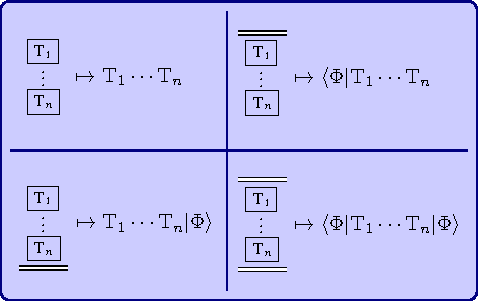
\includegraphics[height=5.7cm]{figs/diagram-ordering.pdf}
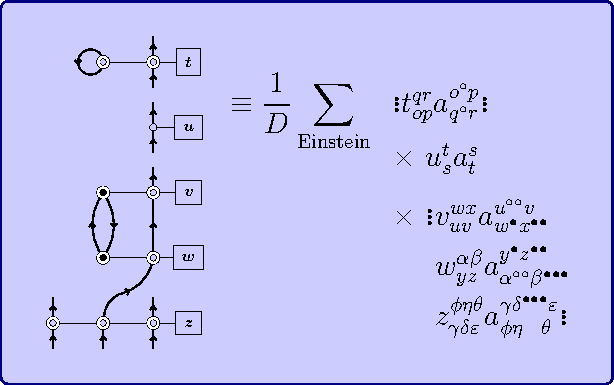
\includegraphics[height=5.7cm]{figs/diagram-example.pdf}
\caption{(a) vertical ordering of a diagram, showing four possible cases of vacuum state bra/ket bookends.
(b)~a~generic example of a diagram, along with its corresponding algebraic term.}
\end{figure}

\begin{ex}
The degeneracy of the product in fig~\ref{fig:diagram-example}(b) is $D=2!2!3!$, so the diagram's degeneracy factor is $\sfr{1}{D}=\sfr{1}{24}$.
\end{ex}

\begin{ex}
Applying the rules of interpretation to a single un-contracted Goldstone operator: 1.~tells us that all lines are summed over, 3.~tells us that the expression has a factor of $\dfr{1}{(m!)^2}$ in front
\begin{align*}
&&
\diagram{
  \node[draw] (label) at (-0.7,0) {\bm{v}};
  \node[dot=white] (v1) at (0,0) {};
  \node[dot=white] (v2) at (1,0) {};
  \node (dots) at (1.75,0) {$\cdots$};
  \node[dot=white] (vn) at (2.5,0) {};
  \draw (label)--(v1)--(v2)--(dots)--(vn);
  \draw[->-] (v1) to ++(0,+0.5);
  \draw[->-] (v2) to ++(0,+0.5);
  \draw[->-] (vn) to ++(0,+0.5);
  \draw[-<-] (v1) to ++(0,-0.5) coordinate[below left=0.1cm and 0.1cm] (startbrace);
  \draw[-<-] (v2) to ++(0,-0.5);
  \draw[-<-] (vn) to ++(0,-0.5) coordinate[below right=0.1cm and 0.1cm] (endbrace);
}
\equiv
  \pr{\tfr{1}{m!}}^2
  \sum_{\substack{p_1\cd p_m\\q_1\cd q_m}}
\diagram{
  \node[draw] (label) at (-0.7,0) {\bm{v}};
  \node[dot=white] (v1) at (0,0) {};
  \node[dot=white] (v2) at (1,0) {};
  \node (dots) at (1.75,0) {$\cdots$};
  \node[dot=white] (vn) at (2.5,0) {};
  \draw (label)--(v1)--(v2)--(dots)--(vn);
  \draw[->-] (v1) to ++(0,+0.45) node[above] {$p_1$};
  \draw[->-] (v2) to ++(0,+0.45) node[above] {$p_2$};
  \draw[->-] (vn) to ++(0,+0.45) node[above] {$p_m$};
  \draw[-<-] (v1) to ++(0,-0.45) node[below] {$q_1$};
  \draw[-<-] (v2) to ++(0,-0.45) node[below] {$q_2$};
  \draw[-<-] (vn) to ++(0,-0.45) node[below] {$q_m$};
}
\equiv&\
  \pr{\tfr{1}{m!}}^2
  \sum_{\text{Einstein}}
  \ol{v}_{p_1p_2\cdots p_m}^{q_1q_2\cdots q_m}
  a^{p_1p_2\cdots p_m}_{q_1q_2\cdots q_m}
\end{align*}
which shows that the diagram is exactly equal to $V$, including the correct summations and the correct scalar factor.
\end{ex}

\begin{ex}
Similarly, for a diagram consisting of a single Hugenholtz operator, we get
\begin{align*}
&&
\diagram{
  \node[draw,circle] (label) at (0,0) {\bm{v}};
  \draw[->-] (label.140) -- ++(140:0.5);
  \draw[->-] (label.120) -- ++(120:0.5);
  \draw[->-] (label.40)  -- ++(40:0.5);
  \node at (70:0.55) {$\cdot$};
  \node at (80:0.55) {$\cdot$};
  \node at (90:0.55) {$\cdot$};
  \draw[-<-] (label.220) -- ++(220:0.5);
  \draw[-<-] (label.240) -- ++(240:0.5);
  \node at (270:0.55) {$\cdot$};
  \node at (280:0.55) {$\cdot$};
  \node at (290:0.55) {$\cdot$};
  \draw[-<-] (label.320) -- ++(320:0.5);
}
\equiv
  \pr{\tfr{1}{m!}}^2
  \sum_{\substack{p_1\cd p_m\\q_1\cd q_m}}
\diagram{
  \node[draw,circle] (label) at (0,0) {\bm{v}};
  \draw[->-] (label.140) -- ++(140:0.5) ++(140:0.2) node {$p_1$};
  \draw[->-] (label.120) -- ++(120:0.5) ++(120:0.2) node {$p_2$};
  \node at (70:0.55) {$\cdot$};
  \node at (80:0.55) {$\cdot$};
  \node at (90:0.55) {$\cdot$};
  \draw[->-] (label.40)  -- ++(40:0.5)  ++(40:0.25)  node {$p_m$};
  \draw[-<-] (label.220) -- ++(220:0.5) ++(220:0.2) node {$q_1$};
  \draw[-<-] (label.240) -- ++(240:0.5) ++(240:0.2) node {$q_2$};
  \node at (270:0.55) {$\cdot$};
  \node at (280:0.55) {$\cdot$};
  \node at (290:0.55) {$\cdot$};
  \draw[-<-] (label.320) -- ++(320:0.5) ++(320:0.25) node {$q_m$};
}
\equiv
  \pr{\tfr{1}{m!}}^2
  \sum_{\text{Einstein}}
  \ol{v}_{p_1p_2\cdots p_m}^{q_1q_2\cdots q_m}
  a^{p_1p_2\cdots p_m}_{q_1q_2\cdots q_m}
\end{align*}
where we have assigned dummy indices of summation in left-to-right order.
\end{ex}



\begin{dfn}
\thmtitle{External and internal lines}
An \textit{external line} is an un-labeled line connected to a single $m$-electron operator, whereas an \textit{internal line} is an un-labeled line connecting one  $m$-electron operator to another.
\end{dfn}

\begin{dfn}
\thmtitle{Equivalent lines}
Two un-labeled lines with the same direction and orientation are called \textit{equivalent} if they are (a) external lines leaving or entering the same $m$-electron operator, or (b) internal lines connected leaving the same $m$-electron operator and entering the same $m$-electron operator.
\end{dfn}

\begin{dfn}
\thmtitle{Equivalent operators}
Two copies of the an $m$-electron operator in a diagram are considered \textit{equivalent} if they are connected to the same set of operators in the same way and their external lines match in orientation. 
\end{dfn}

\begin{drv}
\thmtitle{Counting the degeneracy of a diagram}
Consider a connected diagram.
First, suppose a diagram has no repeated $m$-electron operators.
A permutation of the summation symbols associated with a pair of equivalent lines applies a transposition to the operator symbols within the operators that they leave and enter.
Since this operation can be undone using the permutational degrees of freedom of the operator elements, these permutations contribute to the overall degeneracy.
Permutations of the summation symbols associated with inequivalent lines, on the other hand, permute symbols \ul{between} operators and so cannot be undone using their individual permutational degrees of freedom.
Therefore, if $L$ is the set of lines in the diagram and $\{L_1,\cd, L_g\}$ is the partitioning of $L$ into equivalent lines then the degeneracy of the diagram is the following.
\begin{align}
&&
  D
=
  |L_1|!\cd|L_g|!
\end{align}
%$
%  D
%=
%  |L_1|!\cd|L_g|!\,.$
%Now, suppose the diagram has one or more repeated $m$-electron operators.
%For each pair of equivalent operators, simultaneous transpositions of all of the indices on one of these operators with all of the indices on another also contribute to the degeneracy.
%If $O$ is the full set of operators in the diagram and $\{O_1,\cd,O_h\}$ is the partitioning of $O$ into equivalent operators then the total degeneracy of the diagram is
%\begin{align}
%&&
%  D
%=
%  |L_1|!\cd|L_g|!
%  |O_1|!\cd|O_h|!
%\end{align}
\end{drv}

\begin{dfn}
\thmtitle{Redundancy of a contraction pattern}
Given a connected diagram with a specific contraction pattern, the number of distinct contractions that can be transformed into the original contraction pattern by relabeling summation indices and using the permational degrees of freedom of the operator elements is the \textit{redundancy} $R$ of the pattern.
This is equivalent to the number of contributions in a Wick expansion that are equal to the term with the reference term.
\end{dfn}

\begin{drv}
\thmtitle{Counting the redundancy of a contraction pattern}
Imagine forming the contraction pattern of a connected diagram step-by-step.
First, consider diagram in which all of the contractions have been removed.
Partition the set of lines $L$ in this diagram into equivalent lines $\{L_1,\cd,L_g\}$.
Now, partition each $L_i$ into subsets $\{L_i(0),L_i(1),\cd,L_i(g)\}$ where $L_i(0)$ become external lines and $L_i(j)$ are joined and contracted with $L_j(i)$ in the final diagram.
Note that $|L_i(j)|=|L_j(i)|$ and $|L_i(j)|=0$ unless $L_i$ and $L_j$ have compatible orientations.
The number of equivalent partitionings is therefore
\begin{align*}
&&
  \prod_{i=1}^g
  {|L_i| \choose |L_i(0)|, |L_i(1)|, \ld, |L_i(g)|}
\end{align*}
where $\ds{{n \choose k_1,\ld,k_m}}\equiv\dfr{n!}{k_1!\cd k_m!}$ are multinomial coefficients.
Finally, consider joining together these partitioned sets of equivalent lines into contractions.
For each $L_i(j)$-$L_j(i)$ pair, there are $|L_i(j)|!=|L_j(i)|!$ equivalent ways of contracting the lines, so the total redundancy of the contraction pattern is
\begin{align}
&&\nonumber
  R
=&\
  \prod_{i=1}^g
  {|L_i| \choose |L_i(0)|, |L_i(1)|, \ld, |L_i(g)|}
  \times
  \prod_{i=1}^g
  \prod_{j=i+1}^g
  |S_i(j)|!
\\\intertext{which simplifies to the following.}
&&
  R
=&\
  \prod_{i=1}^g
  \fr{|L_i|!}{|L_i(0)|!}
  \pr{
    \prod_{j=1}^{i-1}
    \fr{1}{|L_i(j)|!}
  }
\end{align}
\end{drv}

%\begin{dfn}
%\thmtitle{Quasi-equivalent lines}
%Two lines with the same direction and orientation that are leaving (entering) the same $m$-electron operator and entering (leaving) two particle-hole operator vertices are called \textit{quasiequivalent}.
%\end{dfn}

\begin{thm}
\thmtitle{Wick's theorem for diagrams}
\thmstatement{The Wick expansion of a product of $m$-electron operators is given by a normal-ordered sum over all unique contracted diagrams, each corresponding to a single algebraic term, without any minus signs or scalar factors.}
\thmproof{
  Clearly, every term in the Wick expansion corresponds to a diagram, and no minus sign is necessary because the phase is defined by the contracted operator string.
  Therefore, it remains to be shown that a single unique diagram is equal to the sum over all redundant contractions corresponding to the pattern.
  That is, the final degeneracy factor $\sfr{1}{D'}$ for a given term must be equal to the redundancy $R$ of its contraction pattern times the original degeneracy factor $\sfr{1}{D}$ of the component diagrams.
  Evaluating the latter, we get
\begin{align*}
  \fr{R}{D}
=
  \prod_{i=1}^g
  \fr{|L_i|!}{|L_i(0)|!}
  \pr{
    \prod_{j=1}^{i-1}
    \fr{1}{|L_i(j)|!}
  }
\times
  \pr{
    \prod_{i=1}^g
    |L_i|!
  }^{-1}
=
  \prod_{i=1}^g
  \fr{1}{|L_i(0)|!}
  \pr{
    \prod_{j=1}^{i-1}
    \fr{1}{|L_i(j)|!}
  }
\end{align*}
  but $\{L_i(0)\}\cup\{L_i(j)\,|\,j<i\}$ is precisely equal the partitioning of the final diagram into equivalent lines, so
\begin{align*}
  D'
=
  \prod_{i=1}^g
  |L_i(0)|!
  \pr{
    \prod_{j=1}^{i-1}
    |L_i(j)|!
  }
=
  \fr{D}{R}
\end{align*}
  which completes the proof.
}
\end{thm}


\begin{dfn}
\thmtitle{Adjacent}
Two that share a vertex are called \textit{adjacent}.
\end{dfn}

\begin{dfn}
\thmtitle{Path}
A sequence of adjacent lines is called a \textit{path}.
Each path has either two external lines, in which case it is an \textit{open path}, or none, in which case it is a \textit{closed path}.
A closed path is also known as a \textit{loop}.
\end{dfn}

\begin{prop}
\thmtitle{Phase factor for a path}
\end{prop}

\begin{cor}
\thmtitle{Phase factor for a loop}
\end{cor}

\begin{cor}
\thmtitle{Phase factor for a completely contracted diagram}
\end{cor}

\begin{ntt}
\thmtitle{Diagram derivatives}
\end{ntt}


%% APPENDICES
\newpage
\appendix
\section{Parenthetical results}

\begin{prop}\label{pull-through-relation}
\thmtitle{Pull-through relation}
\thmstatement{
  For any non-commuting $x_1,\ld,x_n$, and $y$ for which addition, subtraction and multiplication are defined, $x_1\cd x_ny=\pr{\mp}^nyx_1\cd x_n+\sum_{k=1}^n\pr{\mp}^{n-k}x_1\cd[x_k,y]_{\pm}\cd x_n$, where $[x,y]_{\pm}\equiv xy\pm yx$.
}
\thmproof{
  The $n=1$ case folows from the definition of the commutator brackets: $xy=\mp yx+[x,y]_{\pm}$.
  Now, assume it holds for $n$ and consider the $n+1$ case.
  Since $x_1\cd x_{n+1}y=x_1\cd x_n(\mp yx_{n+1}+[x_{n+1},y]_{\pm})$, we find
  \begin{align*}
    x_1\cd x_{n+1}y
  =&\
  \mp
    \pr{
      \pr{\mp}^nyx_1\cd x_n
    +
      \sum_{k=1}^n
      \pr{\mp}^{n-k}
      x_1\cd [x_k,y]_{\pm}\cd x_n
    }
    x_{n+1}
  +
    x_1\cd x_n[x_{n+1},y]_{\pm}
  \\=&\
    \pr{\mp}^{n+1}
    yx_1\cd x_{n+1}
  +
    \sum_{k=1}^{n+1}
    \pr{\mp}^{n+1-k}
    x_1\cd[x_k,y]_{\pm}\cd x_{n+1}
  \end{align*}
  and, by induction, the result holds for all $n$.
}
\end{prop}

\begin{prop}\label{m-electron-operators-ordinary-and-antisymmetrized}
\thmtitle{Expressing $m$-electron operators in terms of ordinary and antisymmetrized integrals}
\thmstatement{
A first-quantized $m$-electron operator $\op{V}=\sum_{i_1<\cd<i_m}\op{v}(i_1\cd i_m)$ can be expressed in two equivalent second-quantized forms
\begin{align*}
  V
=
  \fr{1}{m!}
  \sum_{\substack{p_1\cd p_m\\q_1\cd q_m}}
  \ip{p_1\cd p_m|\op{v}|q_1\cd q_m}
  a_{p_1}\dg\cd a_{p_m}\dg a_{q_m}\cd a_{q_1}
=
  \pr{\fr{1}{m!}}^2
  \sum_{\substack{p_1\cd p_m\\q_1\cd q_m}}
  \ip{p_1\cd p_m|\op{v}|q_{[1}\cd q_{m]}}\,
  a_{p_1}\dg\cd a_{p_m}\dg
  a_{q_m}\cd a_{q_1}
\end{align*}
where
$
  \ip{p_1\cd p_m|\op{v}|q_{[1}\cd q_{m]}}
\equiv
  \sum
  \e_{\pi}
  \ip{p_1\cd p_m|\op{v}|q_{\pi(1)}\cd q_{\pi(m)}}
$
are antisymmetrized $m$-electron integrals
and the original $m$-electron integrals are given by
$\ip{p_1\cd p_m|\op{v}|q_1\cd q_m}\equiv\int d(1\cd m)\y_{p_1}^*(1)\cd \y_{p_m}^*(m)\op{v}(1\cd m)\y_{q_1}(1)\cd \y_{q_m}(m)$.
}
\thmproof{
  It follows from \Cref{direct-derivation-of-second-quantization} that any function $\Y$ in Fock space can be decomposed as
  \begin{align*}
    \Y(1,\cd,n)
  =
    \fr{1}{\sqrt{m!}}
    \sum_{p_1\cd p_m}
    \y_{p_1}(1)\cd\y_{p_m}(m)
    (\op{a}_{p_m}\cd\op{a}_{p_1}\Y)(m,\cd,n)
  \end{align*}
  and therefore the following holds for all $\Y,\Y'\in F(\mc{H})$
  \begin{align*}
    \ip{\Y|\op{V}\Y'}
  =
    \sum_{i_1<\cd<i_m}^n
    \ip{\Y|\op{v}(i_1\cd i_m)\Y'}
  =&\
    \fr{n!}{m!(n-m)!}
    \ip{\Y|\op{v}(1\cd m)\Y'}
  \\=&\
    \fr{1}{m!}
    \sum_{\substack{p_1\cd p_m\\q_1\cd q_m}}^\infty
    \ip{p_1\cd p_m|\op{v}|q_1\cd q_m}
    \ip{\op{a}_{p_m}\cd\op{a}_{p_1}\Y|\op{a}_{q_m}\cd\op{a}_{q_1}\Y'}
  \end{align*}
  which gives the first part of the proposition.
  \begin{align*}
    V
  =
    \fr{1}{m!}
    \sum_{\substack{p_1\cd p_m\\q_1\cd q_m}}
    \ip{p_1\cd p_m|\op{v}|q_1\cd q_m}
    a_{p_1}\dg\cd a_{p_m}\dg a_{q_m}\cd a_{q_1}
  \end{align*}
  The antisymmetrized form can then be derived by the following rearrangement
  \begin{align*}
    V
  =&\
    \fr{1}{m!}
    \sum_{\substack{p_1\cd p_m\\q_1\cd q_m}}
    \ip{p_1\cd p_m|\op{v}|q_1\cd q_m}\,
    a_{p_1}\dg\cd a_{p_m}\dg a_{q_m}\cd a_{q_1}
  \\=&\
    \pr{\fr{1}{m!}}^2
    \sum_{\substack{p_1\cd p_m\\q_1\cd q_m}}
    \sum_{\pi\in\mr{S}_m}
    \ip{p_1\cd p_m|\op{v}|q_{\pi(1)}\cd q_{\pi(m)}}\,
    a_{p_1}\dg\cd a_{p_m}\dg
    a_{q_{\pi(m)}}\cd a_{q_{\pi(1)}}
  \\=&\
    \pr{\fr{1}{m!}}^2
    \sum_{\substack{p_1\cd p_m\\q_1\cd q_m}}
    \sum_{\pi\in\mr{S}_m}
    \e_{\pi}
    \ip{p_1\cd p_m|\op{v}|q_{\pi(1)}\cd q_{\pi(m)}}\,
    a_{p_1}\dg\cd a_{p_m}\dg
    a_{q_m}\cd a_{q_1}
  \end{align*}
  where the first step follows from simply relabeling the dummy indices of summation $q_1\cd q_m$ in $m!$ different ways and the second step follows from the fact that annihilation operators anticommute with other annihilation operators.
}
\end{prop}

\end{document}